% Converted from appendix_recordings.md by scripts/md_to_latex.py; edit this file.
% DRAFT v0.1 (2026-10-08). Appendices for Part A: individual recordings (A), recording
% quality and walking detection (B), visual check of spots (C).
% Numbers from outputs/recordings/<rec>/ (impact_stats.json, impacts_by_road.csv,
% fms_match_rates.csv), outputs/sensor_validity/ and outputs/combined/; figures copied to
% paper/figures/appendix/ by scripts/paper_part_a.py. Full methods: SENSOR_VALIDITY.md,
% SPOT_CHECK.md.

\section{Individual recordings}\label{individual-recordings}

The main text reports the three rides together. This appendix gives each ride on its
own. Hotspots here are numbered separately within each ride (impacts within 30 m of
each other in that ride); the spots P1--P33 of the main text are formed from the pooled
impacts and are numbered differently. Rates per km are left blank (--) where less than
0.2 km was ridden on a road.

% outputs/recordings/<rec>/impact_stats.json

\begin{longtable}[]{@{}
  >{\raggedright\arraybackslash}p{(\linewidth - 6\tabcolsep) * \real{0.2500}}
  >{\raggedright\arraybackslash}p{(\linewidth - 6\tabcolsep) * \real{0.2500}}
  >{\raggedright\arraybackslash}p{(\linewidth - 6\tabcolsep) * \real{0.2500}}
  >{\raggedright\arraybackslash}p{(\linewidth - 6\tabcolsep) * \real{0.2500}}@{}}
\caption{Impacts per ride.}\label{tab:A1}\tabularnewline
\toprule\noalign{}
\begin{minipage}[b]{\linewidth}\raggedright
\end{minipage} & \begin{minipage}[b]{\linewidth}\raggedright
Ride 1
\end{minipage} & \begin{minipage}[b]{\linewidth}\raggedright
Ride 2
\end{minipage} & \begin{minipage}[b]{\linewidth}\raggedright
Ride 3
\end{minipage} \\
\midrule\noalign{}
\endfirsthead
\toprule\noalign{}
\begin{minipage}[b]{\linewidth}\raggedright
\end{minipage} & \begin{minipage}[b]{\linewidth}\raggedright
Ride 1
\end{minipage} & \begin{minipage}[b]{\linewidth}\raggedright
Ride 2
\end{minipage} & \begin{minipage}[b]{\linewidth}\raggedright
Ride 3
\end{minipage} \\
\midrule\noalign{}
\endhead
\bottomrule\noalign{}
\endlastfoot
Date, start (local) & 3 Oct, 18:30 & 7 Oct, 10:37 & 7 Oct, 13:38 \\
Vehicle (Voiager 5) & SZ22 & UPAR & BTLZ \\
Distance ridden & 2.89 km & 1.48 km & 1.71 km \\
Riding time; mean riding speed & 9.6 min; 18.1 km/h & 5.9 min; 15.1 km/h & 6.3 min; 16.4 km/h \\
Impacts (per km; metres between) & 40 (13.8; 72 m) & 39 (26.4; 38 m) & 21 (12.3; 81 m) \\
Median peak (interquartile range) & 1.19 g (1.13--1.35) & 1.34 g (1.19--1.77) & 1.67 g (1.13--1.85) \\
Maximum & 2.80 g & 2.87 g & 6.28 g \\
≥ 1.5 g; ≥ 2.0 g & 6; 4 & 15; 3 & 11; 5 \\
Marked wobble; also ≥ 1.5 g & 13; 3 & 11; 5 & 8; 4 \\
Speed vs peak, Spearman ρ (p) & 0.03 (0.88) & −0.63 (\textless{} 0.001) & −0.68 (0.001) \\
Hotspots within the ride (2+ impacts) & 11 & 6 & 3 \\
\end{longtable}

% outputs/recordings/<rec>/impacts_by_road.csv

\begin{longtable}[]{@{}
  >{\raggedright\arraybackslash}p{(\linewidth - 6\tabcolsep) * \real{0.2500}}
  >{\raggedright\arraybackslash}p{(\linewidth - 6\tabcolsep) * \real{0.2500}}
  >{\raggedright\arraybackslash}p{(\linewidth - 6\tabcolsep) * \real{0.2500}}
  >{\raggedright\arraybackslash}p{(\linewidth - 6\tabcolsep) * \real{0.2500}}@{}}
\caption{Impacts per km by road and ride (km ridden in brackets).}\label{tab:A2}\tabularnewline
\toprule\noalign{}
\begin{minipage}[b]{\linewidth}\raggedright
Road
\end{minipage} & \begin{minipage}[b]{\linewidth}\raggedright
Ride 1
\end{minipage} & \begin{minipage}[b]{\linewidth}\raggedright
Ride 2
\end{minipage} & \begin{minipage}[b]{\linewidth}\raggedright
Ride 3
\end{minipage} \\
\midrule\noalign{}
\endfirsthead
\toprule\noalign{}
\begin{minipage}[b]{\linewidth}\raggedright
Road
\end{minipage} & \begin{minipage}[b]{\linewidth}\raggedright
Ride 1
\end{minipage} & \begin{minipage}[b]{\linewidth}\raggedright
Ride 2
\end{minipage} & \begin{minipage}[b]{\linewidth}\raggedright
Ride 3
\end{minipage} \\
\midrule\noalign{}
\endhead
\bottomrule\noalign{}
\endlastfoot
Marston Road & 11.6 (0.95 km) & 15.8 (0.82 km) & 9.3 (0.75 km) \\
Morrell Avenue & 12.2 (0.98 km) & -- (0.04 km, 3 impacts) & -- (0.03 km, 0 impacts) \\
Old Road & 8.2 (0.24 km) & not ridden & not ridden \\
Headington Road & not ridden & -- (0.02 km, 1 impact) & not ridden \\
Other roads & 21.0 (0.72 km) & 36.7 (0.60 km) & 15.1 (0.93 km) \\
\end{longtable}

% outputs/recordings/<rec>/fms_match_rates.csv

\begin{longtable}[]{@{}
  >{\raggedright\arraybackslash}p{(\linewidth - 6\tabcolsep) * \real{0.2500}}
  >{\raggedright\arraybackslash}p{(\linewidth - 6\tabcolsep) * \real{0.2500}}
  >{\raggedright\arraybackslash}p{(\linewidth - 6\tabcolsep) * \real{0.2500}}
  >{\raggedright\arraybackslash}p{(\linewidth - 6\tabcolsep) * \real{0.2500}}@{}}
\caption{Impacts with a road-surface FixMyStreet report made in the 365 days before the ride within 15, 25 and 50 m, against the same share for all points on the ridden route (baseline).}\label{tab:A3}\tabularnewline
\toprule\noalign{}
\begin{minipage}[b]{\linewidth}\raggedright
Radius
\end{minipage} & \begin{minipage}[b]{\linewidth}\raggedright
Ride 1: impacts / baseline
\end{minipage} & \begin{minipage}[b]{\linewidth}\raggedright
Ride 2: impacts / baseline
\end{minipage} & \begin{minipage}[b]{\linewidth}\raggedright
Ride 3: impacts / baseline
\end{minipage} \\
\midrule\noalign{}
\endfirsthead
\toprule\noalign{}
\begin{minipage}[b]{\linewidth}\raggedright
Radius
\end{minipage} & \begin{minipage}[b]{\linewidth}\raggedright
Ride 1: impacts / baseline
\end{minipage} & \begin{minipage}[b]{\linewidth}\raggedright
Ride 2: impacts / baseline
\end{minipage} & \begin{minipage}[b]{\linewidth}\raggedright
Ride 3: impacts / baseline
\end{minipage} \\
\midrule\noalign{}
\endhead
\bottomrule\noalign{}
\endlastfoot
15 m & 5.0\% / 7.7\% & 15.4\% / 20.7\% & 28.6\% / 19.4\% \\
25 m & 5.0\% / 14.3\% & 30.8\% / 32.7\% & 42.9\% / 34.3\% \\
50 m & 17.5\% / 28.2\% & 69.2\% / 53.1\% & 66.7\% / 54.0\% \\
\end{longtable}

% outputs/recordings/<rec>/fms_match_rates.csv (any-date columns)
\begin{table}[htbp]
\centering\small
\caption{As Table~\ref{tab:A3}, but with FixMyStreet road-surface reports of any date since 2009. Most route points lie near some report, so these shares measure report density rather than reporting of the impacts; this is why the main comparison uses only the 365 days before each ride.}\label{tab:A3any}
\begin{tabular}{@{}lrrr@{}}
\toprule
Radius & Ride 1: impacts / baseline & Ride 2: impacts / baseline & Ride 3: impacts / baseline \\
\midrule
15 m & 42.5\% / 52.3\% & 84.6\% / 75.0\% & 81.0\% / 74.2\% \\
25 m & 62.5\% / 70.3\% & 87.2\% / 84.9\% & 100.0\% / 87.0\% \\
50 m & 72.5\% / 85.9\% & 89.7\% / 93.8\% & 100.0\% / 94.1\% \\
\bottomrule
\end{tabular}
\end{table}

Each ride was compared with reports downloaded for its own route's area (ride 1 on
3 October 2026, rides 2 and 3 on 8 October 2026). In ride 1, none of the six impacts of
1.5 g or more and one of its eleven hotspots had a recent report within 25 m.

\textbf{Notes per ride.}

\begin{itemize}
\tightlist
\item
  \textbf{Ride 1.} One hotspot (near 51.7522, −1.2377; spot P12 in the main text) was hit on
  three separate passes, up to 2.68 g. It lies 6 m from a pothole reported in January
  2026 and marked ``fixed''. The two strongest impacts (2.80 g and 2.68 g) came at low
  speed just after a stop.
\item
  \textbf{Ride 2.} Thirteen impacts followed each other every 0.6--1.2 s at about 8 km/h over
  roughly 20 m (spot P3). The ride ended at 10:46 (Voi rental end); the walk that
  followed is excluded by the speed rule (Appendix B).
\item
  \textbf{Ride 3.} The strongest impact of all rides, 6.28 g at 8.1 km/h, was followed by four
  more impacts of 1.8--3.0 g within about 4 s (spot P4).
\end{itemize}

\FloatBarrier
\subsection{Ride 1 figures}

\begin{figure}
\centering
{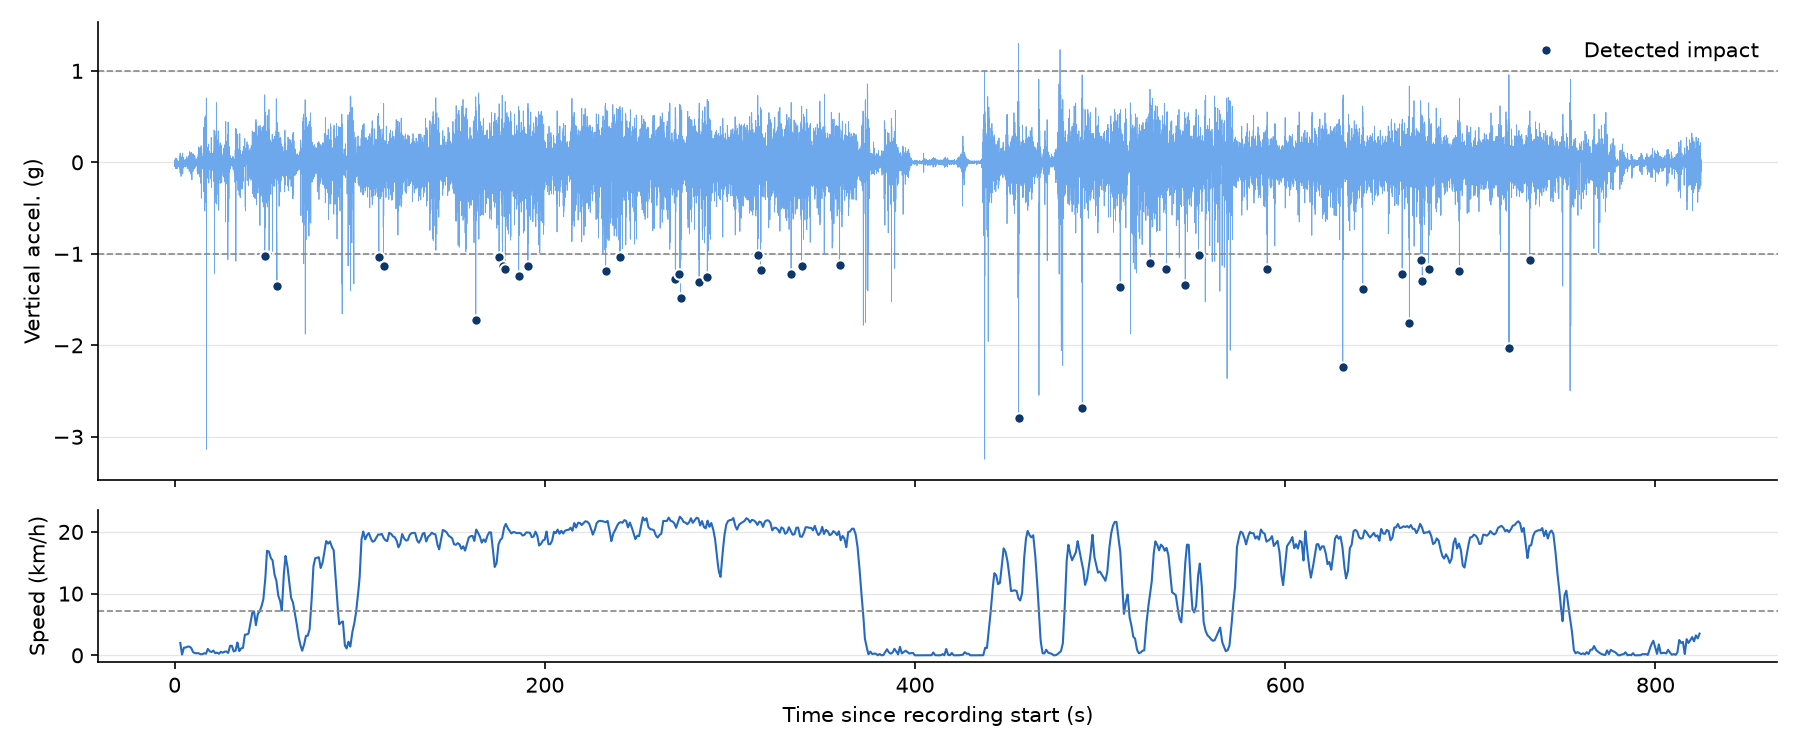
\includegraphics[width=\linewidth]{appendix/2026-10-03_1830_rec01_impact_trace.png}}
\caption{Ride 1: vertical acceleration (top) and GPS speed (bottom) over the recording, with detected impacts. Dashed lines: ±1 g threshold and 7 km/h speed rule.}\label{fig:A1}
\end{figure}

\begin{figure}
\centering
{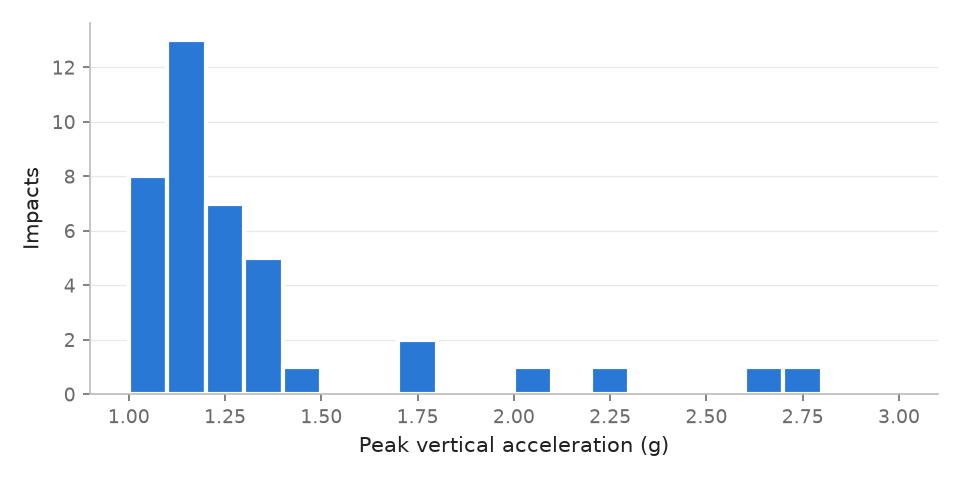
\includegraphics[width=\linewidth]{appendix/2026-10-03_1830_rec01_fig_severity_hist.png}}
\caption{Ride 1: peak vertical acceleration of the 40 impacts.}\label{fig:A2}
\end{figure}

\begin{figure}
\centering
{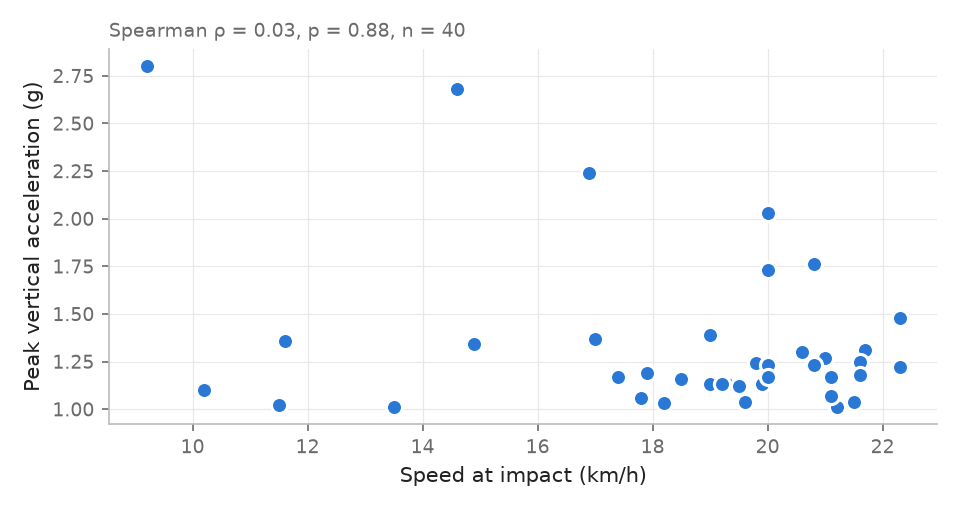
\includegraphics[width=\linewidth]{appendix/2026-10-03_1830_rec01_fig_speed_vs_severity.png}}
\caption{Ride 1: GPS speed against peak vertical acceleration for each impact. One ride; no trend is claimed.}\label{fig:A3}
\end{figure}

\begin{figure}
\centering
{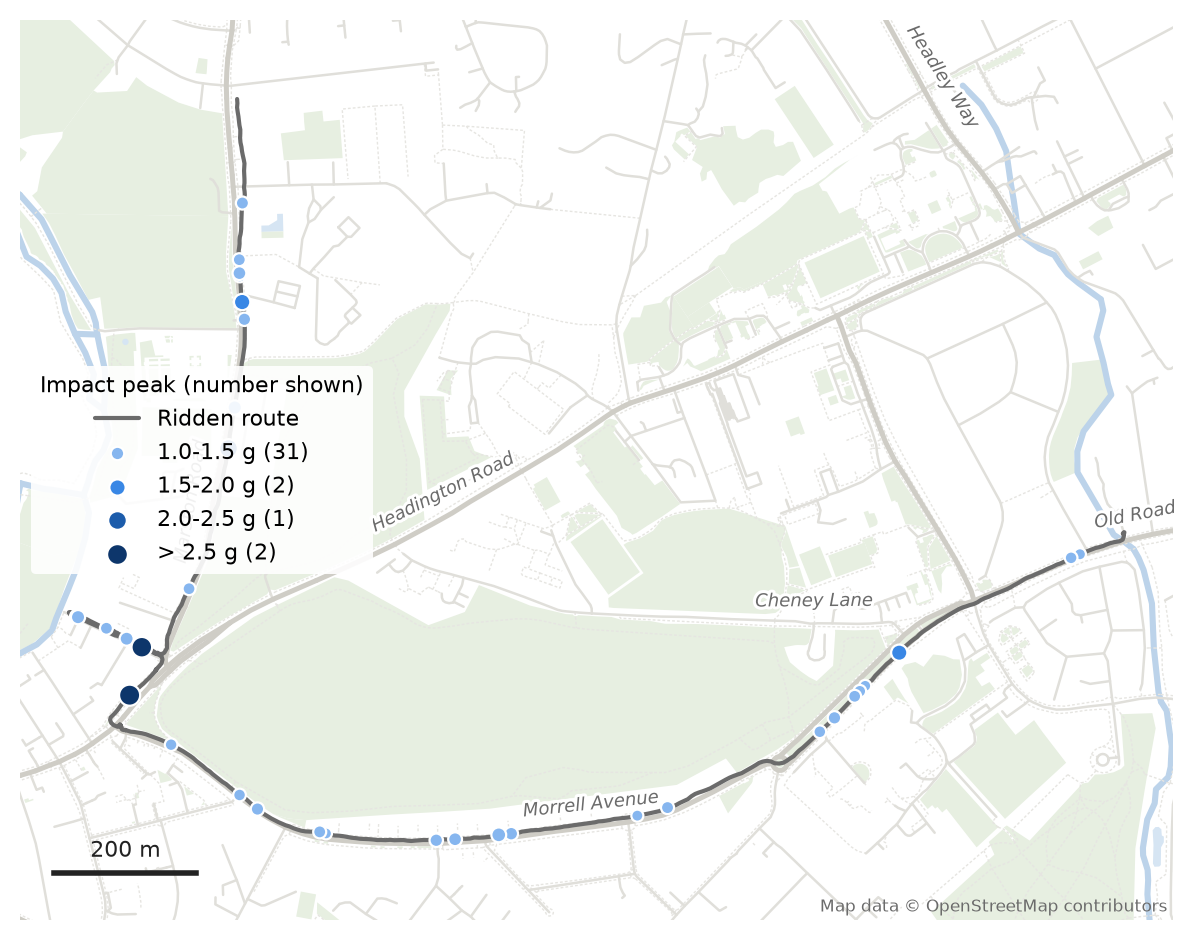
\includegraphics[width=\linewidth]{appendix/2026-10-03_1830_rec01_impact_map.png}}
\caption{Ride 1: impacts on the ridden route, coloured by severity band (bands are analyst choices). Route ends (200 m) and impacts or reports near them are not drawn, for privacy; such impacts are still counted in Table~\ref{tab:A1}. Map data \copyright{} OpenStreetMap contributors.}\label{fig:A4}
\end{figure}

\begin{figure}
\centering
{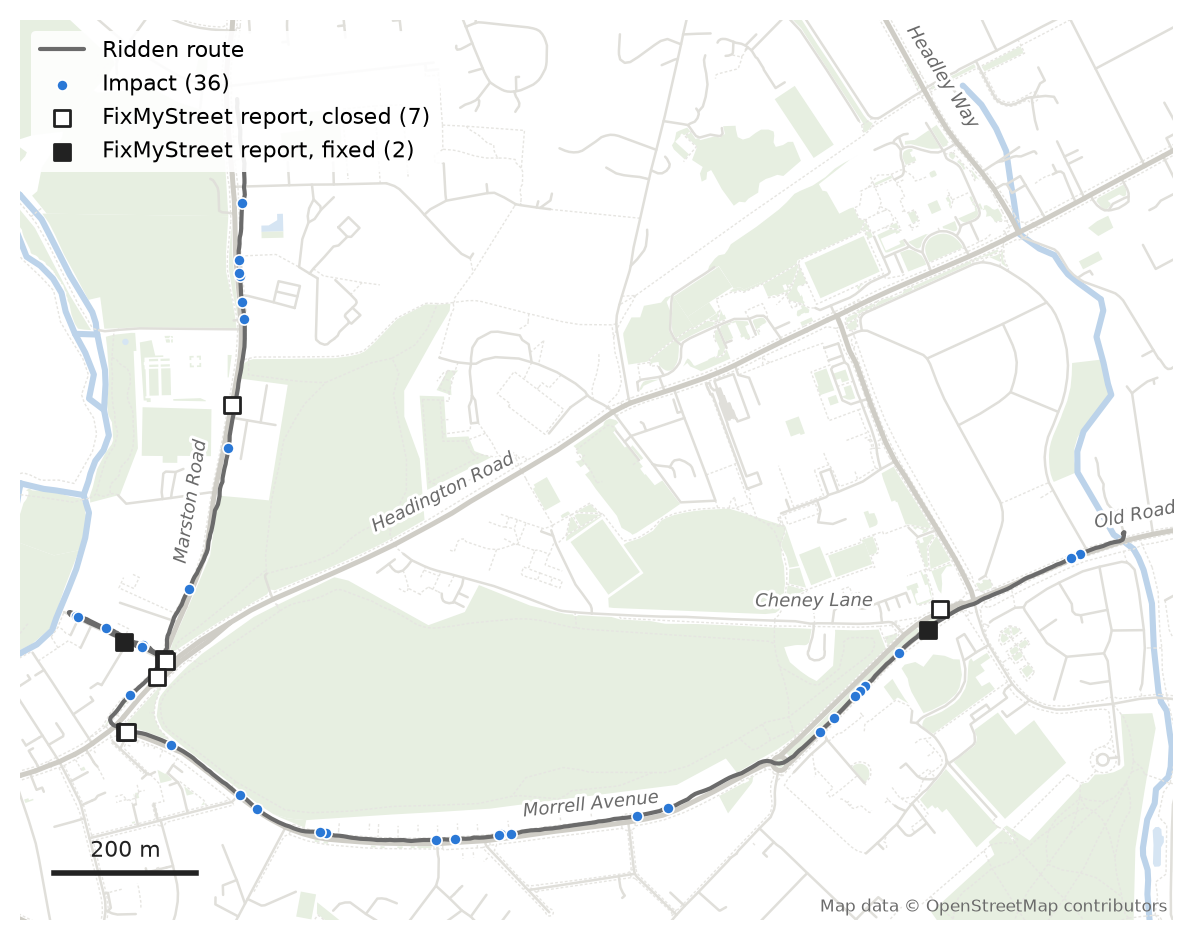
\includegraphics[width=\linewidth]{appendix/2026-10-03_1830_rec01_fms_map.png}}
\caption{Ride 1: impacts and FixMyStreet road-surface reports made in the 365 days before the ride (hollow: closed; filled: marked fixed). A report near an impact does not show that it refers to the same defect. Route ends (200 m) and impacts or reports near them are not drawn, for privacy; such impacts are still counted in Table~\ref{tab:A1}. Map data \copyright{} OpenStreetMap contributors.}\label{fig:A5}
\end{figure}

\FloatBarrier
\subsection{Ride 2 figures}

\begin{figure}
\centering
{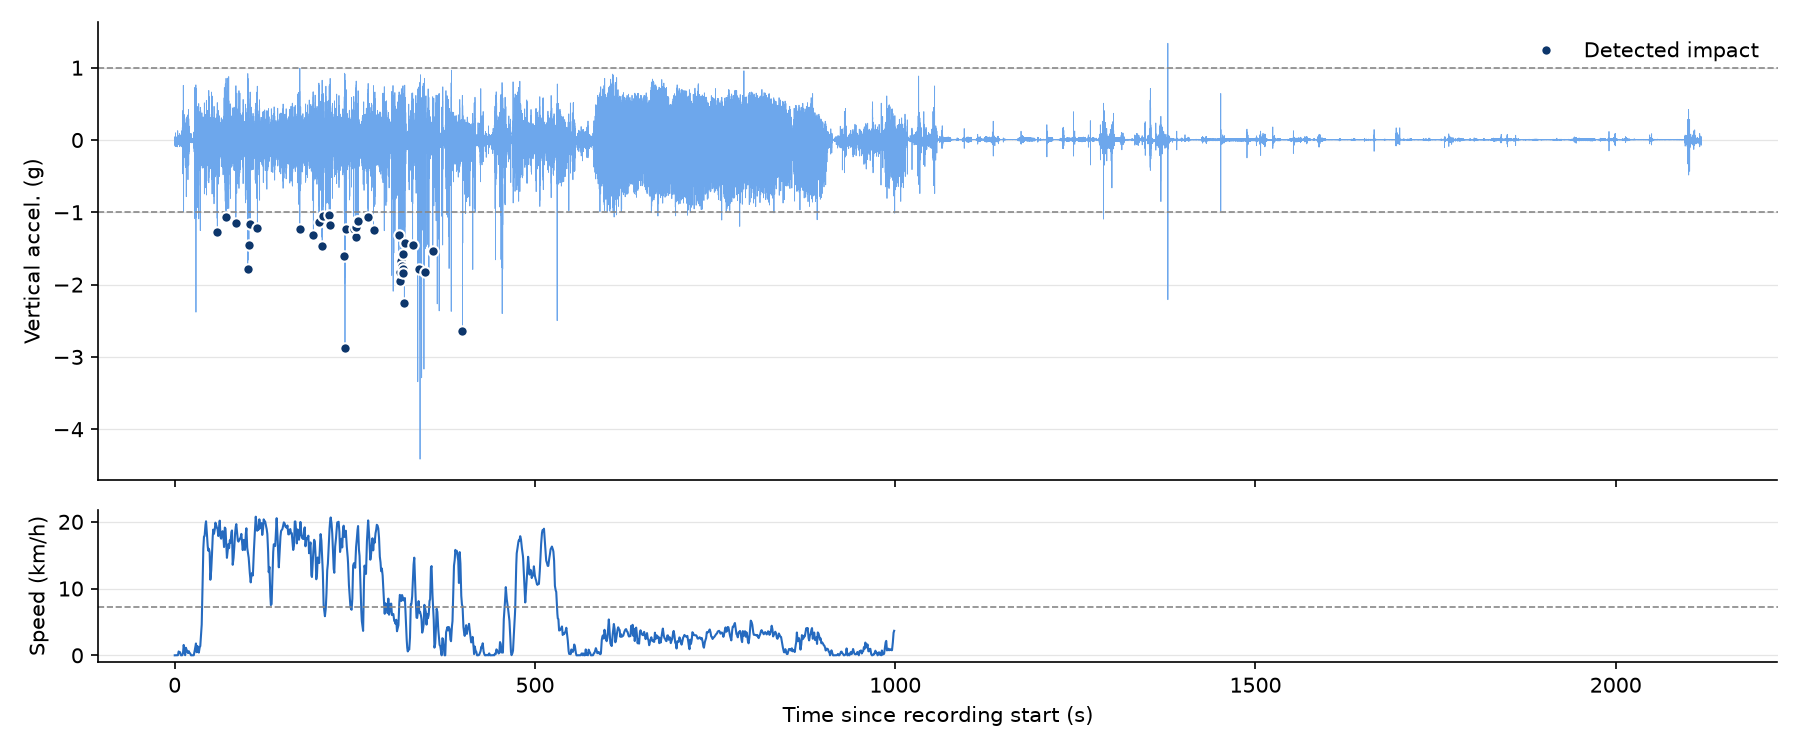
\includegraphics[width=\linewidth]{appendix/2026-10-07_1037_rec02_impact_trace.png}}
\caption{Ride 2: vertical acceleration (top) and GPS speed (bottom) over the recording, with detected impacts. The walk (about 580--900 s) and the phone at rest afterwards produce no impacts because of the speed rule.}\label{fig:A6}
\end{figure}

\begin{figure}
\centering
{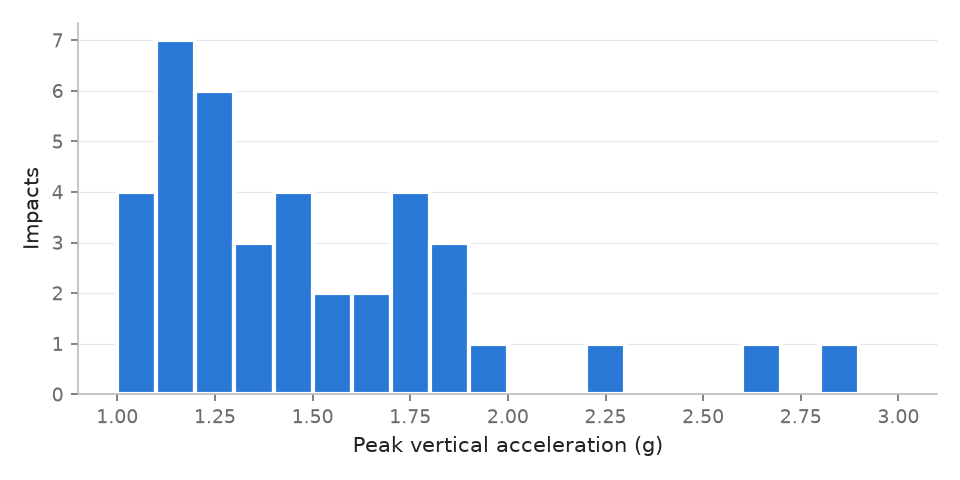
\includegraphics[width=\linewidth]{appendix/2026-10-07_1037_rec02_fig_severity_hist.png}}
\caption{Ride 2: peak vertical acceleration of the 39 impacts.}\label{fig:A7}
\end{figure}

\begin{figure}
\centering
{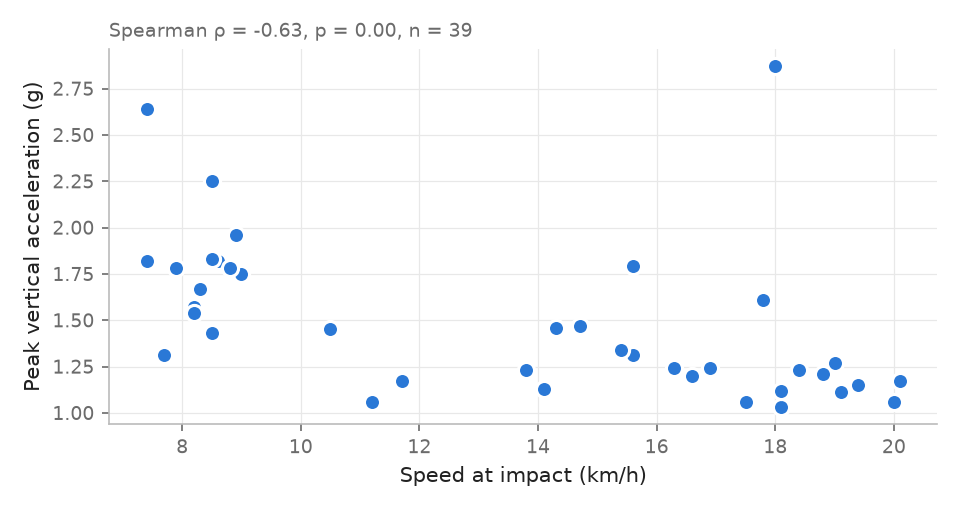
\includegraphics[width=\linewidth]{appendix/2026-10-07_1037_rec02_fig_speed_vs_severity.png}}
\caption{Ride 2: GPS speed against peak vertical acceleration for each impact. One ride; no trend is claimed.}\label{fig:A8}
\end{figure}

\begin{figure}
\centering
{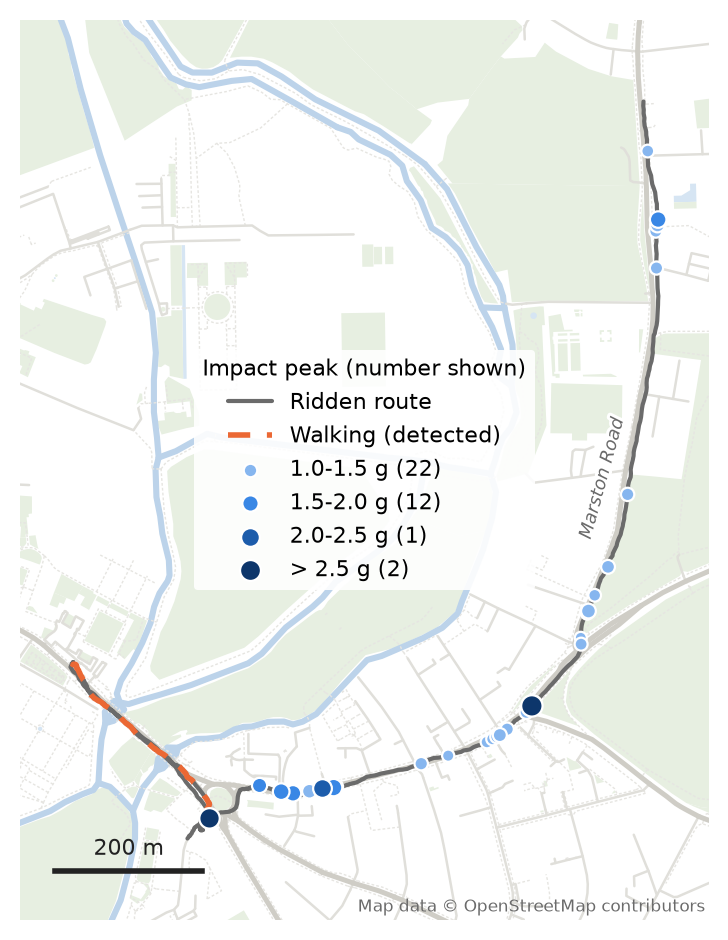
\includegraphics[width=\linewidth]{appendix/2026-10-07_1037_rec02_impact_map.png}}
\caption{Ride 2: impacts on the ridden route, coloured by severity band (bands are analyst choices). The dashed orange line is the walk detected in Appendix~B (not ridden; no impacts are counted there). Route ends (200 m) and impacts or reports near them are not drawn, for privacy; such impacts are still counted in Table~\ref{tab:A1}. Map data \copyright{} OpenStreetMap contributors.}\label{fig:A9}
\end{figure}

\begin{figure}
\centering
{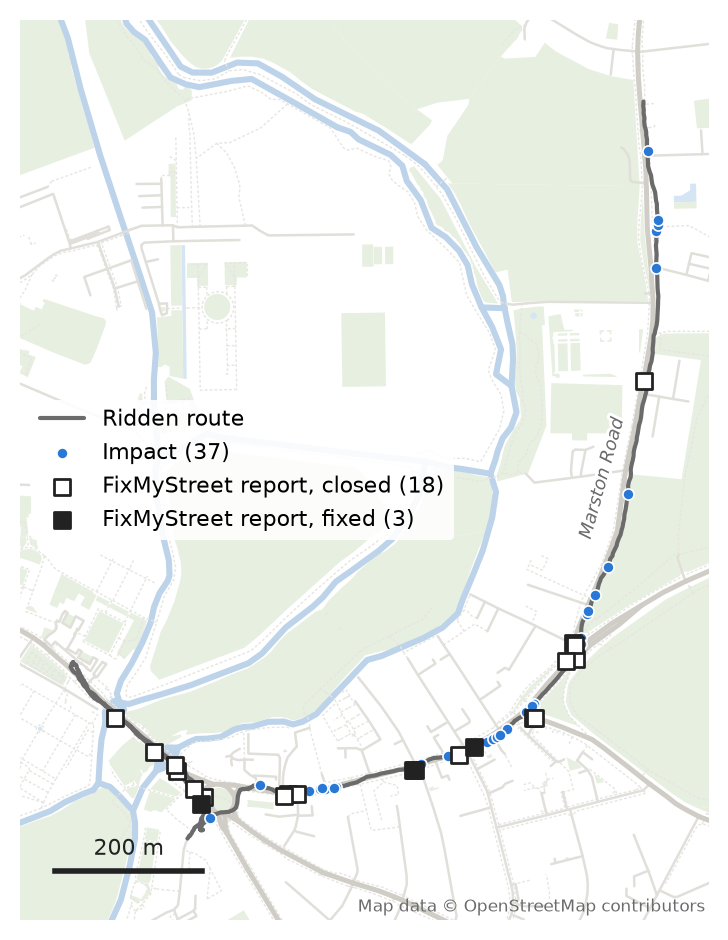
\includegraphics[width=\linewidth]{appendix/2026-10-07_1037_rec02_fms_map.png}}
\caption{Ride 2: impacts and FixMyStreet road-surface reports made in the 365 days before the ride (hollow: closed; filled: marked fixed). A report near an impact does not show that it refers to the same defect. Route ends (200 m) and impacts or reports near them are not drawn, for privacy; such impacts are still counted in Table~\ref{tab:A1}. Map data \copyright{} OpenStreetMap contributors.}\label{fig:A10}
\end{figure}

\FloatBarrier
\subsection{Ride 3 figures}

\begin{figure}
\centering
{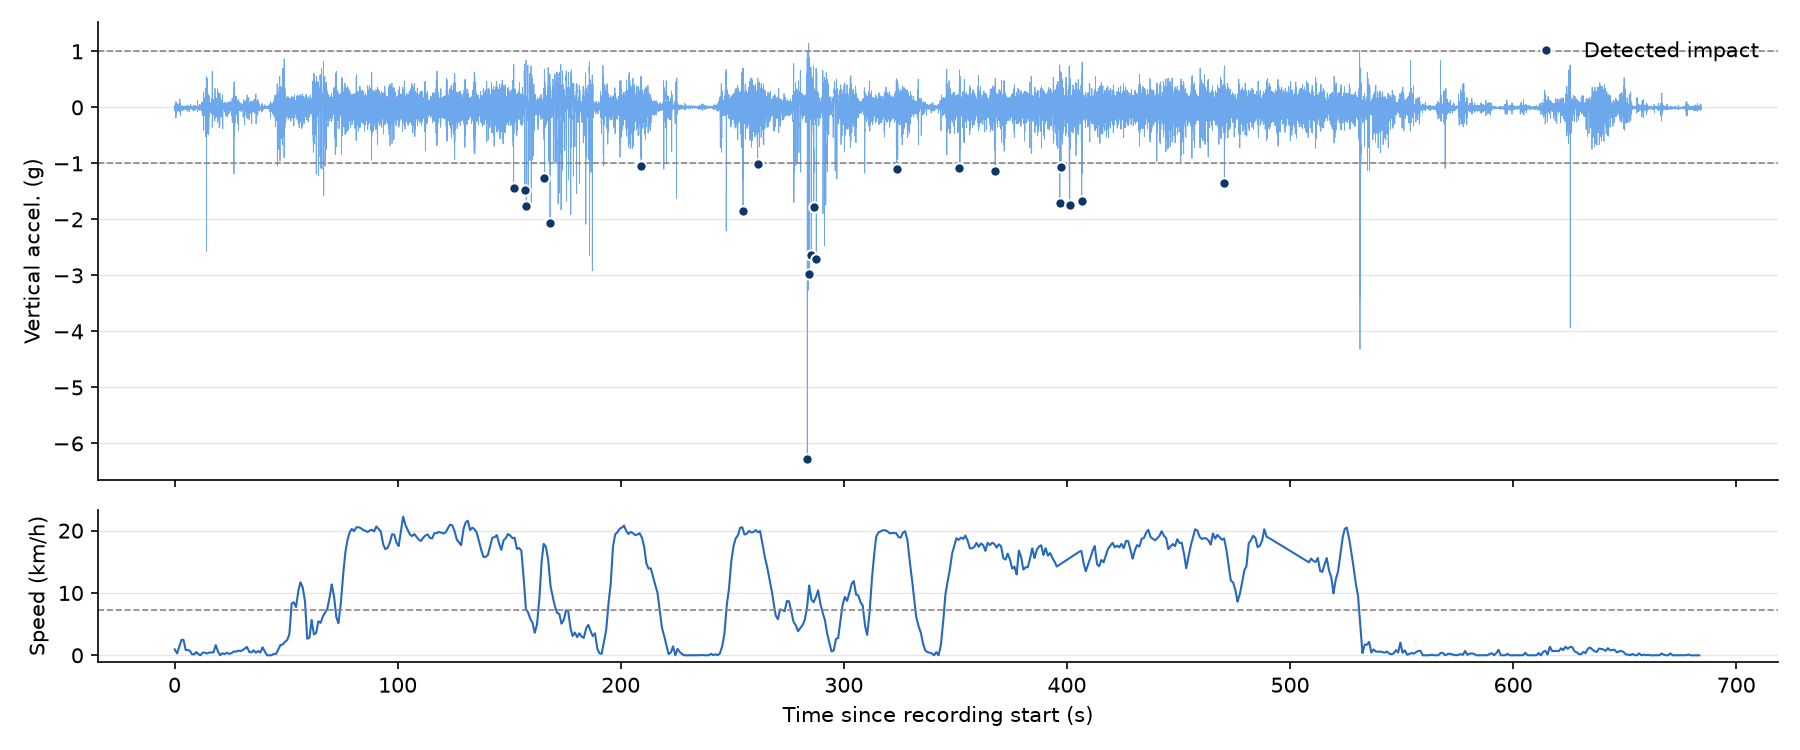
\includegraphics[width=\linewidth]{appendix/2026-10-07_1338_rec03_impact_trace.png}}
\caption{Ride 3: vertical acceleration (top) and GPS speed (bottom) over the recording, with detected impacts.}\label{fig:A11}
\end{figure}

\begin{figure}
\centering
{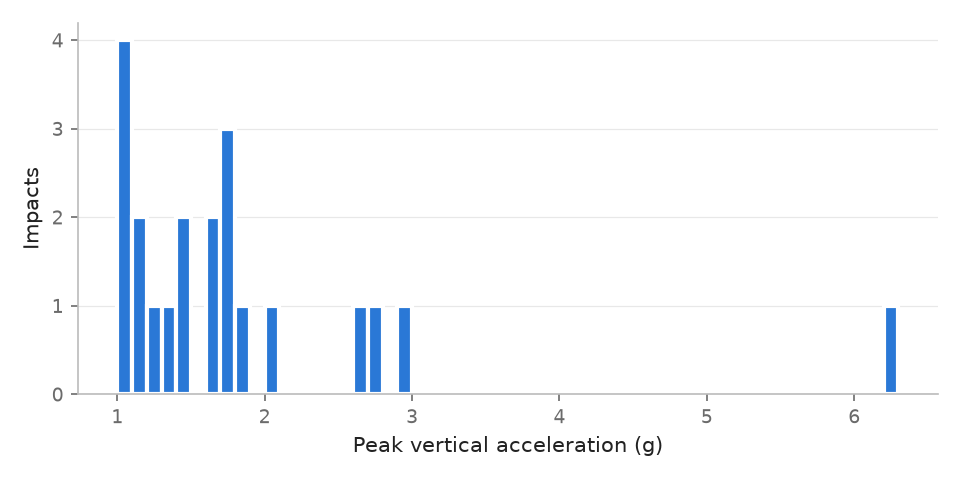
\includegraphics[width=\linewidth]{appendix/2026-10-07_1338_rec03_fig_severity_hist.png}}
\caption{Ride 3: peak vertical acceleration of the 21 impacts.}\label{fig:A12}
\end{figure}

\begin{figure}
\centering
{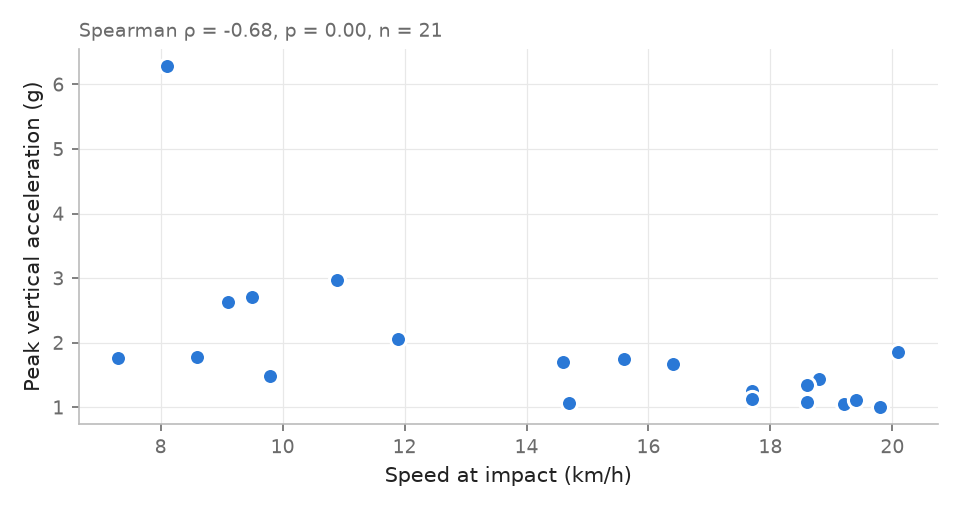
\includegraphics[width=\linewidth]{appendix/2026-10-07_1338_rec03_fig_speed_vs_severity.png}}
\caption{Ride 3: GPS speed against peak vertical acceleration for each impact. One ride; no trend is claimed.}\label{fig:A13}
\end{figure}

\begin{figure}
\centering
{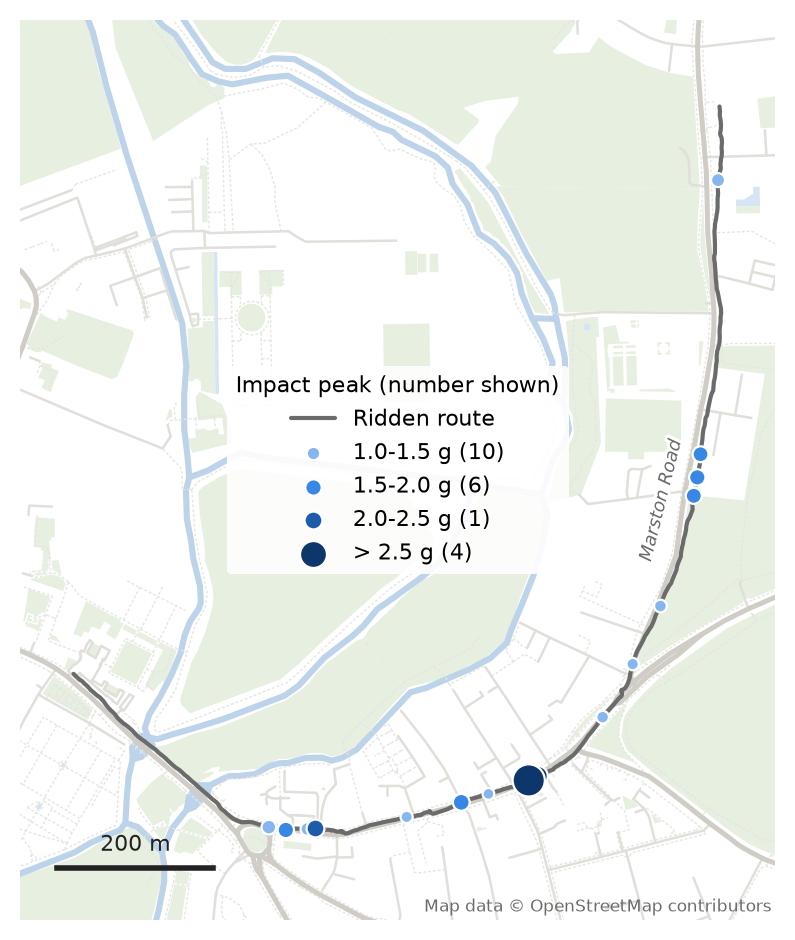
\includegraphics[width=\linewidth]{appendix/2026-10-07_1338_rec03_impact_map.png}}
\caption{Ride 3: impacts on the ridden route, coloured by severity band (bands are analyst choices). Route ends (200 m) and impacts or reports near them are not drawn, for privacy; such impacts are still counted in Table~\ref{tab:A1}. Map data \copyright{} OpenStreetMap contributors.}\label{fig:A14}
\end{figure}

\begin{figure}
\centering
{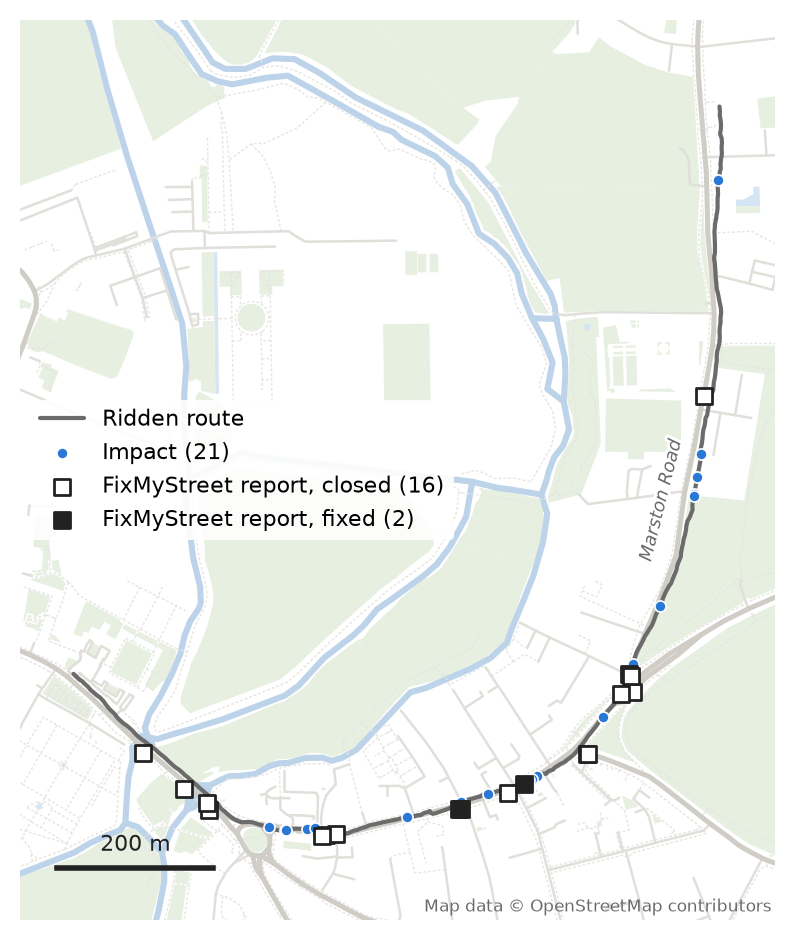
\includegraphics[width=\linewidth]{appendix/2026-10-07_1338_rec03_fms_map.png}}
\caption{Ride 3: impacts and FixMyStreet road-surface reports made in the 365 days before the ride (hollow: closed; filled: marked fixed). A report near an impact does not show that it refers to the same defect. Route ends (200 m) and impacts or reports near them are not drawn, for privacy; such impacts are still counted in Table~\ref{tab:A1}. Map data \copyright{} OpenStreetMap contributors.}\label{fig:A15}
\end{figure}

\FloatBarrier
\subsection{All impacts}
% outputs/combined/impacts_all.csv, outputs/combined/spot_links.csv
\begingroup\small
\begin{longtable}{@{}rrlrrllll@{}}
\caption{All 100 detected impacts. Time is local (Europe/London); speed is GPS speed at the impact; wobble = gyroscope ratio $\geq$ 1.5 after vs before (an analyst choice); report = a FixMyStreet road-surface report made in the 365 days before the ride within 25 m; spot = location in Table~\ref{tab:C1} (spots P9, P16, P30 and P31 lie in the trimmed route ends and have no location there). Coordinates are not listed, for privacy; the anonymised dataset is described under Data availability.}\label{tab:Aimpacts}\\
\toprule
Ride & \# & Time & Peak (g) & Speed (km/h) & Wobble & Road & Report $\leq$25 m & Spot \\
\midrule
\endfirsthead
\toprule
Ride & \# & Time & Peak (g) & Speed (km/h) & Wobble & Road & Report $\leq$25 m & Spot \\
\midrule
\endhead
\bottomrule
\endlastfoot
1 & 1 & 18:31:17 & 1.02 & 11.5 &  & Other roads &  & P16 \\
1 & 2 & 18:31:24 & 1.36 & 11.6 & yes & Other roads &  & P16 \\
1 & 3 & 18:32:19 & 1.04 & 19.6 & yes & Old Road &  & P20 \\
1 & 4 & 18:32:21 & 1.13 & 19.0 &  & Old Road &  & P20 \\
1 & 5 & 18:33:11 & 1.73 & 20.0 &  & Other roads &  & P22 \\
1 & 6 & 18:33:24 & 1.03 & 18.2 &  & Other roads &  & P14 \\
1 & 7 & 18:33:26 & 1.13 & 19.3 &  & Other roads &  & P14 \\
1 & 8 & 18:33:27 & 1.17 & 21.1 &  & Other roads &  & P14 \\
1 & 9 & 18:33:34 & 1.24 & 19.8 &  & Other roads &  & P18 \\
1 & 10 & 18:33:39 & 1.13 & 19.9 &  & Other roads &  & P18 \\
1 & 11 & 18:34:21 & 1.19 & 21.6 &  & Morrell Avenue &  & P25 \\
1 & 12 & 18:34:29 & 1.04 & 21.5 &  & Morrell Avenue &  & P33 \\
1 & 13 & 18:34:59 & 1.27 & 21.0 & yes & Morrell Avenue &  & P13 \\
1 & 14 & 18:35:01 & 1.22 & 22.3 & yes & Morrell Avenue &  & P13 \\
1 & 15 & 18:35:02 & 1.48 & 22.3 &  & Morrell Avenue &  & P13 \\
1 & 16 & 18:35:12 & 1.31 & 21.7 & yes & Morrell Avenue &  & P17 \\
1 & 17 & 18:35:16 & 1.25 & 21.6 &  & Morrell Avenue &  & P17 \\
1 & 18 & 18:35:44 & 1.01 & 21.2 & yes & Morrell Avenue &  & P19 \\
1 & 19 & 18:35:45 & 1.18 & 21.6 &  & Morrell Avenue &  & P19 \\
1 & 20 & 18:36:02 & 1.23 & 20.0 &  & Morrell Avenue &  & P24 \\
1 & 21 & 18:36:07 & 1.13 & 19.2 &  & Morrell Avenue &  & P28 \\
1 & 22 & 18:36:28 & 1.12 & 19.5 &  & Morrell Avenue &  & P29 \\
1 & 23 & 18:38:05 & 2.80 & 9.2 & yes & Other roads &  & P8 \\
1 & 24 & 18:38:39 & 2.68 & 14.6 &  & Other roads &  & P12 \\
1 & 25 & 18:38:59 & 1.37 & 17.0 &  & Other roads &  & P15 \\
1 & 26 & 18:39:16 & 1.10 & 10.2 &  & Other roads &  & P15 \\
1 & 27 & 18:39:24 & 1.17 & 17.4 & yes & Other roads &  & P26 \\
1 & 28 & 18:39:35 & 1.34 & 14.9 &  & Other roads & yes & P12 \\
1 & 29 & 18:39:42 & 1.01 & 13.5 &  & Other roads &  & P12 \\
1 & 30 & 18:40:19 & 1.16 & 18.5 & yes & Marston Road &  & P2 \\
1 & 31 & 18:41:00 & 2.24 & 16.9 &  & Marston Road &  & P1 \\
1 & 32 & 18:41:10 & 1.39 & 19.0 &  & Marston Road & yes & P23 \\
1 & 33 & 18:41:32 & 1.23 & 20.8 &  & Marston Road &  & P5 \\
1 & 34 & 18:41:36 & 1.76 & 20.8 & yes & Marston Road &  & P5 \\
1 & 35 & 18:41:42 & 1.07 & 21.1 & yes & Marston Road &  & P5 \\
1 & 36 & 18:41:43 & 1.30 & 20.6 &  & Marston Road &  & P5 \\
1 & 37 & 18:41:46 & 1.17 & 20.0 &  & Marston Road &  & P5 \\
1 & 38 & 18:42:03 & 1.19 & 17.9 & yes & Marston Road &  & P10 \\
1 & 39 & 18:42:29 & 2.03 & 20.0 & yes & Marston Road &  & P9 \\
1 & 40 & 18:42:41 & 1.06 & 17.8 &  & Marston Road &  & P30 \\
\midrule
2 & 1 & 10:38:05 & 1.27 & 19.0 &  & Marston Road &  & P9 \\
2 & 2 & 10:38:17 & 1.06 & 17.5 &  & Marston Road &  & P31 \\
2 & 3 & 10:38:31 & 1.15 & 19.4 & yes & Marston Road &  & P27 \\
2 & 4 & 10:38:47 & 1.79 & 15.6 & yes & Marston Road &  & P5 \\
2 & 5 & 10:38:49 & 1.46 & 14.3 &  & Marston Road &  & P5 \\
2 & 6 & 10:38:51 & 1.17 & 11.7 &  & Marston Road &  & P5 \\
2 & 7 & 10:39:01 & 1.21 & 18.8 &  & Marston Road &  & P5 \\
2 & 8 & 10:40:00 & 1.23 & 18.4 &  & Marston Road &  & P1 \\
2 & 9 & 10:40:18 & 1.31 & 15.6 & yes & Marston Road &  & P2 \\
2 & 10 & 10:40:27 & 1.13 & 14.1 &  & Marston Road &  & P2 \\
2 & 11 & 10:40:31 & 1.47 & 14.7 & yes & Marston Road &  & P2 \\
2 & 12 & 10:40:32 & 1.06 & 11.2 &  & Marston Road &  & P2 \\
2 & 13 & 10:40:40 & 1.03 & 18.1 & yes & Marston Road & yes & P7 \\
2 & 14 & 10:40:42 & 1.17 & 20.1 &  & Headington Road & yes & P7 \\
2 & 15 & 10:41:02 & 1.61 & 17.8 & yes & Morrell Avenue & yes & P11 \\
2 & 16 & 10:41:02 & 2.87 & 18.0 & yes & Morrell Avenue & yes & P11 \\
2 & 17 & 10:41:04 & 1.24 & 16.9 &  & Morrell Avenue & yes & P11 \\
2 & 18 & 10:41:15 & 1.23 & 13.8 &  & Other roads &  & P4 \\
2 & 19 & 10:41:17 & 1.34 & 15.4 & yes & Other roads &  & P4 \\
2 & 20 & 10:41:18 & 1.20 & 16.6 &  & Other roads &  & P4 \\
2 & 21 & 10:41:19 & 1.12 & 18.1 &  & Other roads &  & P4 \\
2 & 22 & 10:41:21 & 1.11 & 19.1 &  & Other roads & yes & P4 \\
2 & 23 & 10:41:34 & 1.06 & 20.0 &  & Other roads & yes & P6 \\
2 & 24 & 10:41:42 & 1.24 & 16.3 & yes & Other roads & yes & P6 \\
2 & 25 & 10:42:18 & 1.31 & 7.7 &  & Other roads &  & P3 \\
2 & 26 & 10:42:19 & 1.96 & 8.9 &  & Other roads &  & P3 \\
2 & 27 & 10:42:19 & 1.82 & 8.6 &  & Other roads &  & P3 \\
2 & 28 & 10:42:21 & 1.67 & 8.3 &  & Other roads &  & P3 \\
2 & 29 & 10:42:21 & 1.75 & 9.0 &  & Other roads &  & P3 \\
2 & 30 & 10:42:22 & 1.78 & 8.8 &  & Other roads &  & P3 \\
2 & 31 & 10:42:23 & 1.83 & 8.5 &  & Other roads &  & P3 \\
2 & 32 & 10:42:24 & 1.57 & 8.2 &  & Other roads &  & P3 \\
2 & 33 & 10:42:25 & 2.25 & 8.5 &  & Other roads &  & P3 \\
2 & 34 & 10:42:26 & 1.43 & 8.5 &  & Other roads &  & P3 \\
2 & 35 & 10:42:36 & 1.45 & 10.5 &  & Other roads & yes & P3 \\
2 & 36 & 10:42:45 & 1.78 & 7.9 &  & Other roads & yes & P3 \\
2 & 37 & 10:42:53 & 1.82 & 7.4 &  & Other roads & yes & P3 \\
2 & 38 & 10:43:04 & 1.54 & 8.2 & yes & Other roads &  & P3 \\
2 & 39 & 10:43:45 & 2.64 & 7.4 & yes & Other roads & yes & P21 \\
\midrule
3 & 1 & 13:41:06 & 1.44 & 18.8 &  & Other roads &  & P3 \\
3 & 2 & 13:41:11 & 1.48 & 9.8 &  & Other roads &  & P3 \\
3 & 3 & 13:41:12 & 1.76 & 7.3 &  & Other roads &  & P3 \\
3 & 4 & 13:41:20 & 1.25 & 17.7 & yes & Other roads & yes & P3 \\
3 & 5 & 13:41:22 & 2.06 & 11.9 &  & Other roads & yes & P3 \\
3 & 6 & 13:42:03 & 1.05 & 19.2 &  & Other roads &  & P32 \\
3 & 7 & 13:42:49 & 1.85 & 20.1 & yes & Other roads & yes & P6 \\
3 & 8 & 13:42:55 & 1.00 & 19.8 &  & Other roads &  & P6 \\
3 & 9 & 13:43:18 & 6.28 & 8.1 & yes & Other roads & yes & P4 \\
3 & 10 & 13:43:19 & 2.97 & 10.9 &  & Other roads & yes & P4 \\
3 & 11 & 13:43:19 & 2.63 & 9.1 &  & Other roads & yes & P4 \\
3 & 12 & 13:43:21 & 1.78 & 8.6 &  & Other roads & yes & P4 \\
3 & 13 & 13:43:22 & 2.71 & 9.5 &  & Other roads & yes & P4 \\
3 & 14 & 13:43:58 & 1.11 & 19.4 & yes & Other roads &  & P8 \\
3 & 15 & 13:44:26 & 1.08 & 18.6 &  & Marston Road & yes & P7 \\
3 & 16 & 13:44:42 & 1.13 & 17.7 & yes & Marston Road &  & P2 \\
3 & 17 & 13:45:11 & 1.70 & 14.6 & yes & Marston Road &  & P1 \\
3 & 18 & 13:45:11 & 1.06 & 14.7 & yes & Marston Road &  & P1 \\
3 & 19 & 13:45:15 & 1.75 & 15.6 & yes & Marston Road &  & P1 \\
3 & 20 & 13:45:21 & 1.67 & 16.4 &  & Marston Road &  & P1 \\
3 & 21 & 13:46:25 & 1.34 & 18.6 &  & Marston Road &  & P10 \\
\end{longtable}
\endgroup



\section{Recording quality and walking detection}\label{recording-quality-and-walking-detection}

% Full version of SENSOR_VALIDITY.md (methods, results, references, limitations);
% numbers from outputs/sensor_validity/ (quality_summary.csv, segments_all.csv,
% walking_onsets.csv, gps_speed_by_activity.csv, ground_truth_comparison.csv, windows.csv).

This appendix gives the full check of the recording method summarised in
section~\ref{checking-the-recording-method}. It tests whether the Sensor Logger data are
internally sound and whether riding can be told apart from walking. Neither part needs a
reference instrument, and neither proves absolute accuracy, which would need a calibrated
accelerometer, survey-grade GNSS or exactly timed events.

\subsection{Methods}

\textbf{Data quality.} Table~\ref{tab:Bchecks} lists the checks, applied to all three
recordings. Units, as checked: user acceleration and gravity are in m/s² in the device
frame \autocite{apple_cmdevicemotion}; the raw accelerometer is in g
\autocite{apple_cmacceleration} (raw ÷ (user acceleration + gravity) = 1/9.80665 on every
axis); the metadata recording time is UTC, so local times were computed from the
nanosecond timestamps.

\begin{table}[htbp]
\centering\small
\caption{Data-quality checks.}\label{tab:Bchecks}
\begin{tabular}{@{}p{30mm}p{72mm}p{50mm}@{}}
\toprule
Check & How & What it can show \\
\midrule
Sampling & Intervals between timestamps: median, 1st and 99th percentile; gaps (more than 1.5 times the nominal interval); out-of-order and duplicate timestamps & Dropped samples, irregular sampling \\
Clock & Absolute timestamp against elapsed time & Disagreeing time bases \\
Raw vs fused acceleration & User acceleration plus gravity, in g and interpolated to the raw sample times, compared with the raw accelerometer & Consistency of the iOS fusion output with the raw sensor (not accuracy) \\
Noise and bias & Quietest 5\% of non-overlapping 4 s windows (by user-acceleration SD): acceleration and gyroscope SD, raw magnitude (1 g at rest), calibrated minus uncalibrated gyroscope mean & Noise and static error if the phone was truly still; otherwise upper bounds \\
Gravity magnitude & Length of the gravity vector & Reported only: fixed at 9.80665 m/s² by the fusion, so not an accuracy test \\
GPS & Fix interval and gaps; reported horizontal accuracy; reported vs position-derived speed; position scatter while standing & Availability, stated precision, internal consistency \\
\bottomrule
\end{tabular}
\end{table}

\textbf{Walking versus riding.} The vertical user acceleration (the projection onto the
gravity direction, up positive \autocite{mizell2003}) was analysed in 4 s windows starting
every 1 s, with the features in Table~\ref{tab:Bfeat}. The rules, applied in order, were:
\emph{stationary} if the vertical SD was below 0.5 m/s² and GPS speed below 2 km/h (or
missing); \emph{walking} if step regularity and step-band share were both at least 0.5 and
GPS speed below 8 km/h (or missing); \emph{riding} if GPS speed was at least 8 km/h and the
step-band share below 0.3; otherwise \emph{unclear} (slow riding, handling the phone,
getting on or off). Labels were smoothed with a centred 5-window majority filter, and a
\emph{walking bout} is at least 10 s of walking windows. All thresholds are analyst choices,
set from physical reasoning and from inspecting ride 2 before the rider's references were
known, not fitted to labels, and not changed afterwards.

\begin{table}[htbp]
\centering\small
\caption{Window features for walking detection.}\label{tab:Bfeat}
\begin{tabular}{@{}p{26mm}p{60mm}p{66mm}@{}}
\toprule
Feature & Definition & Rationale \\
\midrule
Vertical SD & SD of vertical acceleration (m/s²) & Overall motion; near 0 when the phone is still \\
Step-band share & Share of vertical-acceleration power (Welch spectrum \autocite{welch1967}, 256-sample segments) in 1.2--2.8 Hz, out of 0.5--20 Hz & Walking concentrates power at the step frequency (measured means 1.8--2.0 Hz \autocite{pachi2005}; the band is set wider to include slow and brisk walking); scooter vibration is broadband \\
Step regularity & Highest normalised autocorrelation at lags of one step period (0.36--0.83 s) & Measures step regularity and cadence \autocite{moenilssen2004}; steps repeat, vibration does not \\
Cadence & 1 / that lag (steps/s) & Plausibility check \\
GPS speed & Median reported speed of the fixes in the window & Separates riding from walking speed \\
\bottomrule
\end{tabular}
\end{table}

\textbf{Why two acceleration features.} After the walk in ride 2 there are repeated
periods with high step regularity (about 0.85) while the phone is almost still. They have
essentially no power in the step band (share about 0) and tiny amplitude (SD about
0.1 m/s²): a small periodic vibration, not steps (Figure~\ref{fig:B2}). Step regularity
alone would have labelled them walking.

\textbf{First step of a bout.} Vertical acceleration was band-pass filtered (0.8--4 Hz,
second-order Butterworth \autocite{butterworth1930}, applied forwards and backwards for
zero phase shift; SciPy \autocite{virtanen2020scipy}). Steps are peaks with a prominence of
at least 1 m/s², at least 0.35 s apart. From the first step inside the bout, the method
moves back over earlier peaks while successive intervals stay within one step period
(0.35--0.85 s); the earliest peak reached is the first step. The \emph{GPS lag} is the time
from the first step until GPS speed exceeds 1.5 km/h on three consecutive fixes.

\textbf{GPS speed against positions.} Each riding or walking segment of at least 30 s,
trimmed by 15 s at each end, was compared: median reported speed against speed from the
summed fix-to-fix distance (inflated by GPS jitter) and from the straight-line distance
between the first and last fix (a lower bound on the distance travelled). A reported
speed below the straight-line speed under-reads the true speed.

\subsection{Data quality}

\begin{table}[htbp]
\centering\small
\caption{Data quality per recording. Bold: the only recording in which the phone was
truly still (after the walk); in rides 1 and 3 the phone stayed on the handlebar, so the
quietest-window values include vibration and are upper bounds.}\label{tab:Bquality}
\begin{tabular}{@{}p{56mm}p{28mm}p{30mm}p{28mm}@{}}
\toprule
Measure & Ride 1 & Ride 2 & Ride 3 \\
\midrule
Motion sensors: rate & 99.72 Hz & 99.72 Hz & 99.72 Hz \\
Sampling interval, median (99th percentile) & 10.03 (10.03) ms & 10.03 (10.03) ms & 10.03 (10.03) ms \\
Gaps, out-of-order, duplicate timestamps & 0, 0, 0 & 0, 0, 0 & 0, 0, 0 \\
Clock: timestamp vs elapsed time, max difference & 0.0 ms & 0.0 ms & 0.0 ms \\
Raw vs fused acceleration, median (95th pct.) & 0.049 (0.160) g & 0.007 (0.092) g & 0.013 (0.053) g \\
Quietest windows: acceleration SD & 0.31 m/s² & \textbf{0.012 m/s²} & 0.19 m/s² \\
Quietest windows: gyroscope SD & 0.16 rad/s & \textbf{0.0035 rad/s} & 0.095 rad/s \\
Quietest windows: raw magnitude & 1.002 g & \textbf{0.994 g} (SD 0.0009) & 1.003 g \\
Gyroscope calibrated − uncalibrated (x, y, z) & 0.002, 0.005, −0.002 rad/s & 0.002, 0.005, −0.002 rad/s & 0.002, 0.005, −0.002 rad/s \\
GPS fixes; gaps over 1.5 s; longest gap & 828; 2; 17.1 s & 1160; 144; 15.0 s & 686; 0; 1.0 s \\
GPS reported horizontal accuracy, median (90th pct.) & 11.5 (15.1) m & 11.3 (15.5) m & 13.9 (17.6) m \\
GPS position scatter while standing, median (90th pct.) & 0.7 (2.1) m & 0.1 (1.7) m & 0.5 (1.6) m \\
GPS speed: |reported − position-derived|, median & 0.38 m/s & 0.64 m/s & 0.52 m/s \\
\bottomrule
\end{tabular}
\end{table}

\begin{itemize}
\item \emph{Sampling and timing are clean}: no dropped samples, gaps or timestamp faults in
  any motion stream of any recording.
\item \emph{At rest} (ride 2 only), noise is about 0.001 g and the static acceleration
  magnitude is 0.6\% below 1 g, both small against the 1.0 g impact threshold.
\item \emph{Raw and fused acceleration} agree most closely in ride 2 (mostly still) and least
  in ride 1 (riding throughout); likely reasons are fast vibration between samples taken
  at different instants and filtering in the iOS fusion (not tested further).
\item \emph{The gyroscope bias correction} applied by iOS is small and identical across
  recordings (same phone).
\item \emph{GPS horizontal accuracy} (median 11--14 m) is the phone's own estimate, not a
  measured error; for context only, the measured error of an iPhone 6 in an urban area
  averaged 7--13 m \autocite{merry2019}.
\item \emph{GPS gaps}: in ride 2 they start at 10:53:51, after the walk (phone indoors or
  covered); both gaps in ride 1 are at its very start (the first fix is a cached position
  from 17 s before recording began).
\end{itemize}

\subsection{Walking detection}

\begin{table}[htbp]
\centering\small
\caption{Time per label (after smoothing).}\label{tab:Blabels}
\begin{tabular}{@{}lrrrr@{}}
\toprule
Recording & Riding & Walking & Stationary & Unclear \\
\midrule
Ride 1 (ride only) & 564 s & 6 s & 64 s & 187 s \\
Ride 2 (ride, then walk) & 321 s & \textbf{330 s} & 1103 s & 361 s \\
Ride 3 (ride only) & 347 s & 8 s & 100 s & 226 s \\
\bottomrule
\end{tabular}
\end{table}

\begin{table}[htbp]
\centering\small
\caption{Walking bouts detected in ride 2. The two bouts are probably one walk with a
pause of a few seconds around 10:51:21--25 (not confirmed).}\label{tab:Bbouts}
\begin{tabular}{@{}llrrrr@{}}
\toprule
Bout & First step (local time) & Length & Steps & Median cadence & GPS lag at onset \\
\midrule
1 & \textbf{10:46:47.04} (580.6 s into the recording) & 275 s & 562 & 2.04 steps/s & 12.0 s \\
2 & 10:51:25.21 & 37 s & 69 & 1.89 steps/s & 3.8 s \\
\bottomrule
\end{tabular}
\end{table}

\begin{table}[htbp]
\centering\small
\caption{The transition from riding to walking in ride 2 (Figure~\ref{fig:1}).}\label{tab:Btransition}
\begin{tabular}{@{}p{38mm}p{116mm}@{}}
\toprule
Time (approx.) & What the data show \\
\midrule
10:45:52--10:45:57 & GPS speed falls from riding speed, ending in a sharp acceleration spike \\
10:45:58--10:46:06 & A short walking-like burst (8 s, decaying amplitude) \\
10:46:06--10:46:46 & About 40 s of standing or handling the phone (from about 10:46:16 the gravity vector shows the phone lying or held flat) \\
from 10:46:47 & Steady walking \\
\bottomrule
\end{tabular}
\end{table}

The Voi rental ended at 10:46 (app ride history, 10:46:00--10:46:59), which overlaps the
phone-handling period; this is consistent with the rental being ended on the phone then,
but the data cannot show it. The 8 s burst at 10:45:58 resembles the confirmed false
positives below (short, after riding, step regularity below that of the real walk), so
it is not treated as the start of walking.

\textbf{Feature separation} (an independent check). In the 1,126 windows across all three
recordings where GPS speed alone was 12 km/h or more (riding, defined without the
acceleration features), none met the walking criteria: step regularity had a median of
0.18 (maximum 0.45) and step-band share a median of 0.010 (maximum 0.44). In the main
walking bout, step regularity had a median of 0.78 (interquartile range 0.76--0.80) and
step-band share 0.83; these walking values come from the detected bout itself, so they
are not independent of the method.

\begin{table}[htbp]
\centering\small
\caption{Walking labels in the two recordings without walking (rider's confirmation).}\label{tab:Bfp}
\begin{tabular}{@{}lp{52mm}rrr@{}}
\toprule
Recording & Walking labels after smoothing & Before smoothing & Bouts of 10 s+ & At GPS 8 km/h+ \\
\midrule
Ride 1 & 6 s (0.7\% of 821 windows): 18:43:53--55 and 18:44:06--10 & 9 windows & 0 & 0 \\
Ride 3 & 8 s (1.2\% of 681 windows): 13:49:08--16 & 9 windows & 0 & 0 \\
\bottomrule
\end{tabular}
\end{table}

All of these came after the ride had ended, at GPS speeds below 1 km/h, with step
regularity (0.51--0.71) below the real walk's median of 0.78. In ride 1 they fall in the
last 20 s before the recording stopped, with the phone held flat (probably handled); in
ride 3 the phone was roughly in its mounted orientation, about 1.5 min after riding ended.
Their cause (handling the phone, moving or parking the scooter) is not known. The 10 s
minimum bout length was set before the script was first run on rides 1 and 3 and excludes
all of them.

\begin{table}[htbp]
\centering\small
\caption{Detections against the rider's references.}\label{tab:Bref}
\begin{tabular}{@{}lp{42mm}p{24mm}p{58mm}@{}}
\toprule
Recording & Reference (source) & Precision & Detected \\
\midrule
Ride 1 & No walking (rider) & whole recording & 0 walking bouts; 6 s of isolated walking labels after the ride ended \\
Ride 2 & Walking ``after 10 minutes'' = 10:47:06 (rider's recollection) & about a minute & First step of sustained walking 10:46:47.04 (−19 s) \\
Ride 2 & Rental ended 10:46 (Voi app ride history) & one minute & Last riding segment ends 10:45:54; walking starts 10:46:47.04: order consistent \\
Ride 3 & No walking (rider) & whole recording & 0 walking bouts; 8 s of isolated walking labels after the ride ended \\
\bottomrule
\end{tabular}
\end{table}

What the references show: \emph{timing}: two independent references, both with one-minute
precision, place the change from riding to walking in the same minute as the detection,
which is agreement at minute level, not a timing error in seconds; \emph{specificity}:
across about 25 minutes of recordings without walking, no walking bout was detected and
no window was labelled walking while riding; \emph{sensitivity}: there is only one walking
episode, and it was detected, so no detection rate can be given. The rental end marks the
end of the hire, not of riding: the data place riding ending about 6--65 s before it.

\subsection{GPS speed}

\begin{table}[htbp]
\centering\small
\caption{GPS-reported speed against speed from GPS positions (km/h; segments of at least
30 s, 15 s trimmed at each end; the second ride-2 riding segment is 26 s after trimming).
The straight-line speed is a lower bound on the true speed.}\label{tab:Bgps}
\begin{tabular}{@{}llrrr@{}}
\toprule
Ride & Activity & Reported median & Straight-line & Summed path \\
\midrule
1 & riding & 20.1 & 19.0 & 20.8 \\
1 & riding & 19.1 & 19.3 & 19.7 \\
2 & riding & 17.9 & 19.2 & 19.5 \\
2 & riding & 12.1 & 15.3 & 15.4 \\
2 & \textbf{walking} & \textbf{3.0} & \textbf{4.6} & 5.5 \\
3 & riding & 19.5 & 19.5 & 19.6 \\
3 & riding & 17.5 & 19.1 & 19.5 \\
\bottomrule
\end{tabular}
\end{table}

\begin{itemize}
\item \emph{Walking}: the reported speed is at least about 1.5 km/h (34\%) below the
  position-derived lower bound. With the straight-line speed the implied step length is
  at least 4.6 km/h ÷ 2.04 steps/s ≈ 0.62 m, close to measured means of 0.67 m (women) and
  0.75 m (men) \autocite{pachi2005}; with the reported speed it would be 0.41 m.
\item \emph{Riding}: reported and position-derived speeds are closer, but in 4 of 6 segments
  the reported speed is below the straight-line lower bound, by 0.2--3.2 km/h.
\item \emph{Lag}: GPS speed rose about 12 s after walking began (bout 1).
\item \emph{Context}: a dedicated (non-phone) GPS receiver on a bicycle gave speeds within
  0.2 m/s of a calibrated speedometer for 45\% of values, with larger errors on curved
  paths through a tendency to underestimate speed \autocite{witte2004}; phones and walking
  speeds were not tested there.
\item \emph{Consequences for impact detection}: the speed rule is needed, because walking alone
  produced 11 peaks of 1.0 g or more (maximum 1.19 g) and handling the phone after the
  walk 3 more (maximum 2.21 g), none of which were counted. But the rule uses reported
  speed, so some slow-riding impacts may have been excluded (not quantified).
\end{itemize}

\subsection{Limitations of the check}

\begin{itemize}
\item One rider, one phone model, one app version, three recordings, one walking episode
  (about 5 minutes) and about 25 minutes of recordings without walking; other people,
  gaits or phone positions (pocket, bag, walking while pushing the scooter) may behave
  differently.
\item Thresholds are analyst choices set after looking at ride 2; not fitted to labels, but
  not blind either. Rides 1 and 3 were not used to set them.
\item The references have one-minute precision, and the rider's account that rides 1 and 3
  contain no walking is not independently checked.
\item No external reference for acceleration, rotation or position: the data-quality
  results show internal consistency and plausibility, not absolute accuracy.
\item Where the phone was during the walk is not known; the gravity direction was steady
  and similar to the mounted position. Walking with the phone loosely held or in a bag
  may give weaker step signals, which could fall under the stationary rule.
\end{itemize}

\begin{figure}[htbp]
\centering
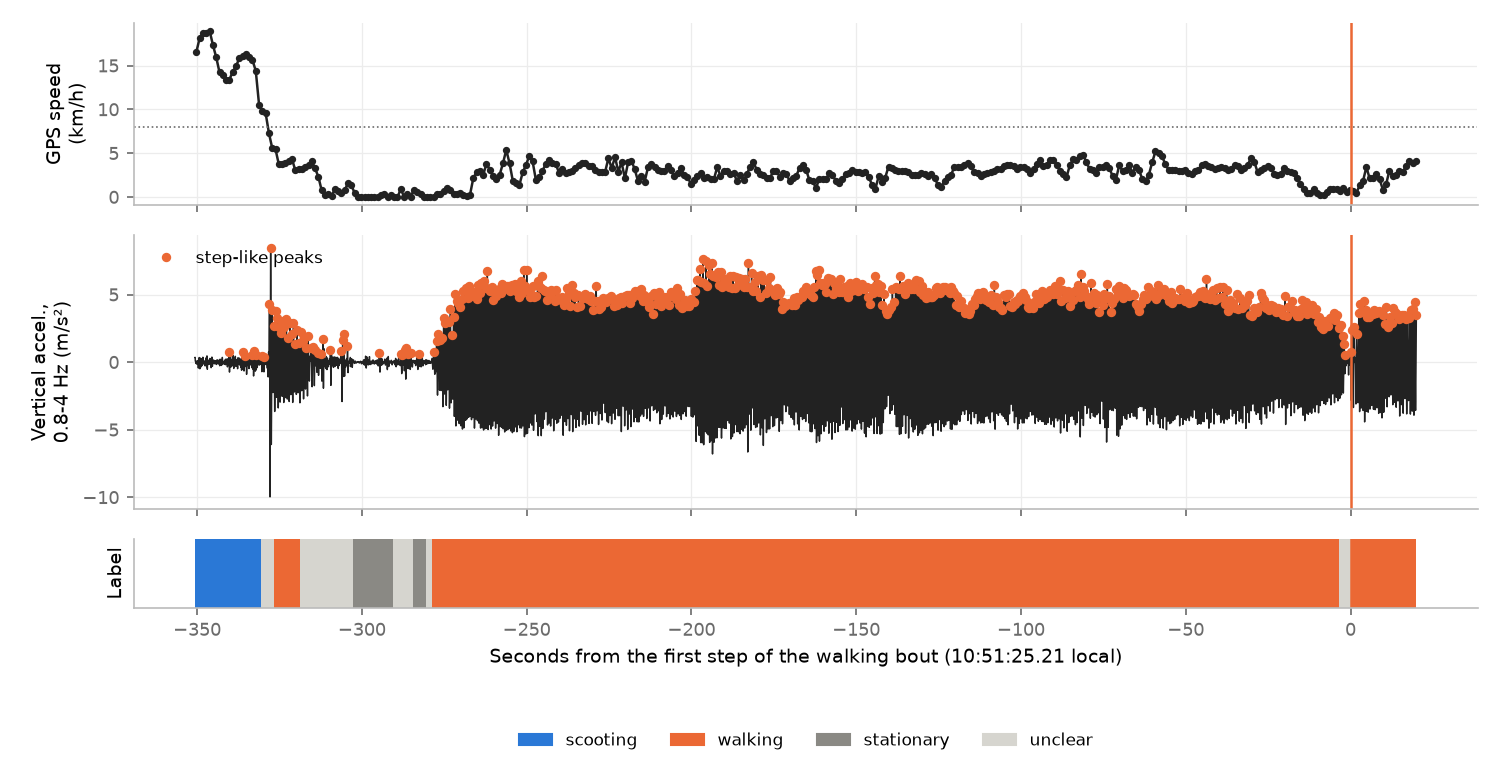
\includegraphics[width=\linewidth]{appendix/2026-10-07_1037_rec02_walk_onset_2.png}
\caption{Start of the second walking bout in ride 2 (first step 10:51:25.21), drawn as
Figure~\ref{fig:1}: GPS speed, band-passed vertical acceleration with step-like peaks, and
window labels.}\label{fig:Bonset2}
\end{figure}

\begin{figure}[htbp]
\centering
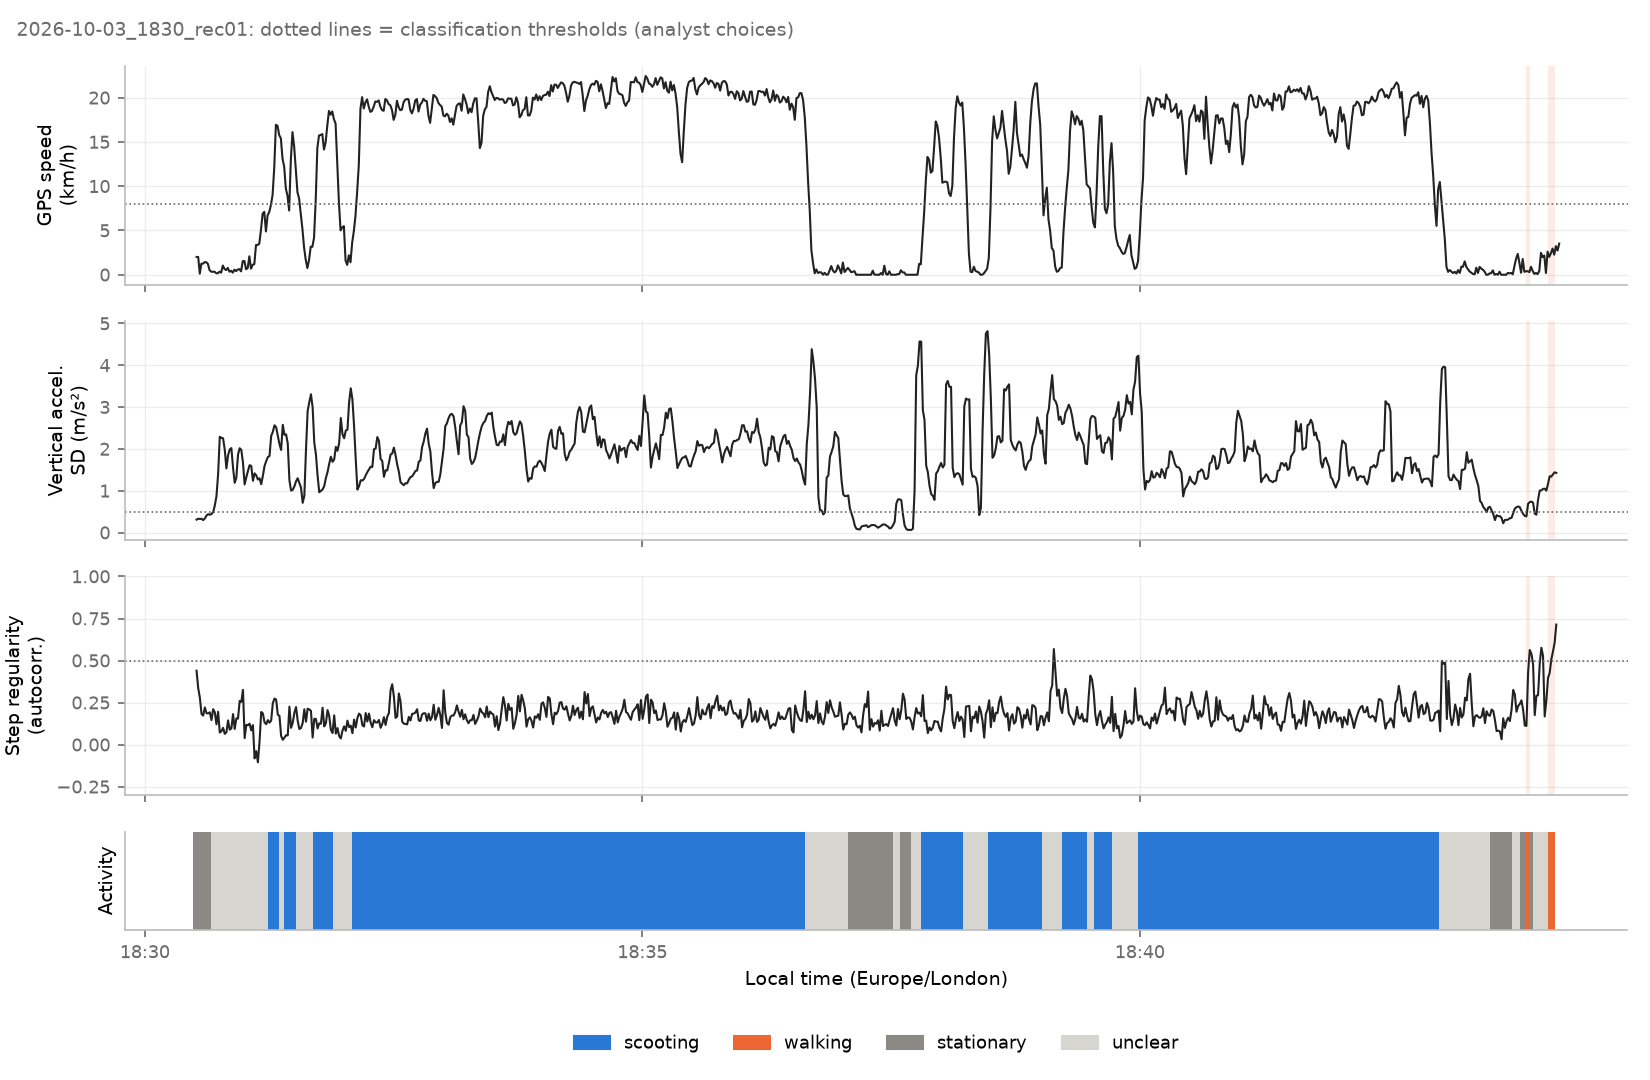
\includegraphics[width=\linewidth]{appendix/2026-10-03_1830_rec01_activity_timeline.png}
\caption{Ride 1: GPS speed, vertical acceleration SD, step regularity and activity
labels. Dotted lines: thresholds.}\label{fig:B1}
\end{figure}

\begin{figure}[htbp]
\centering
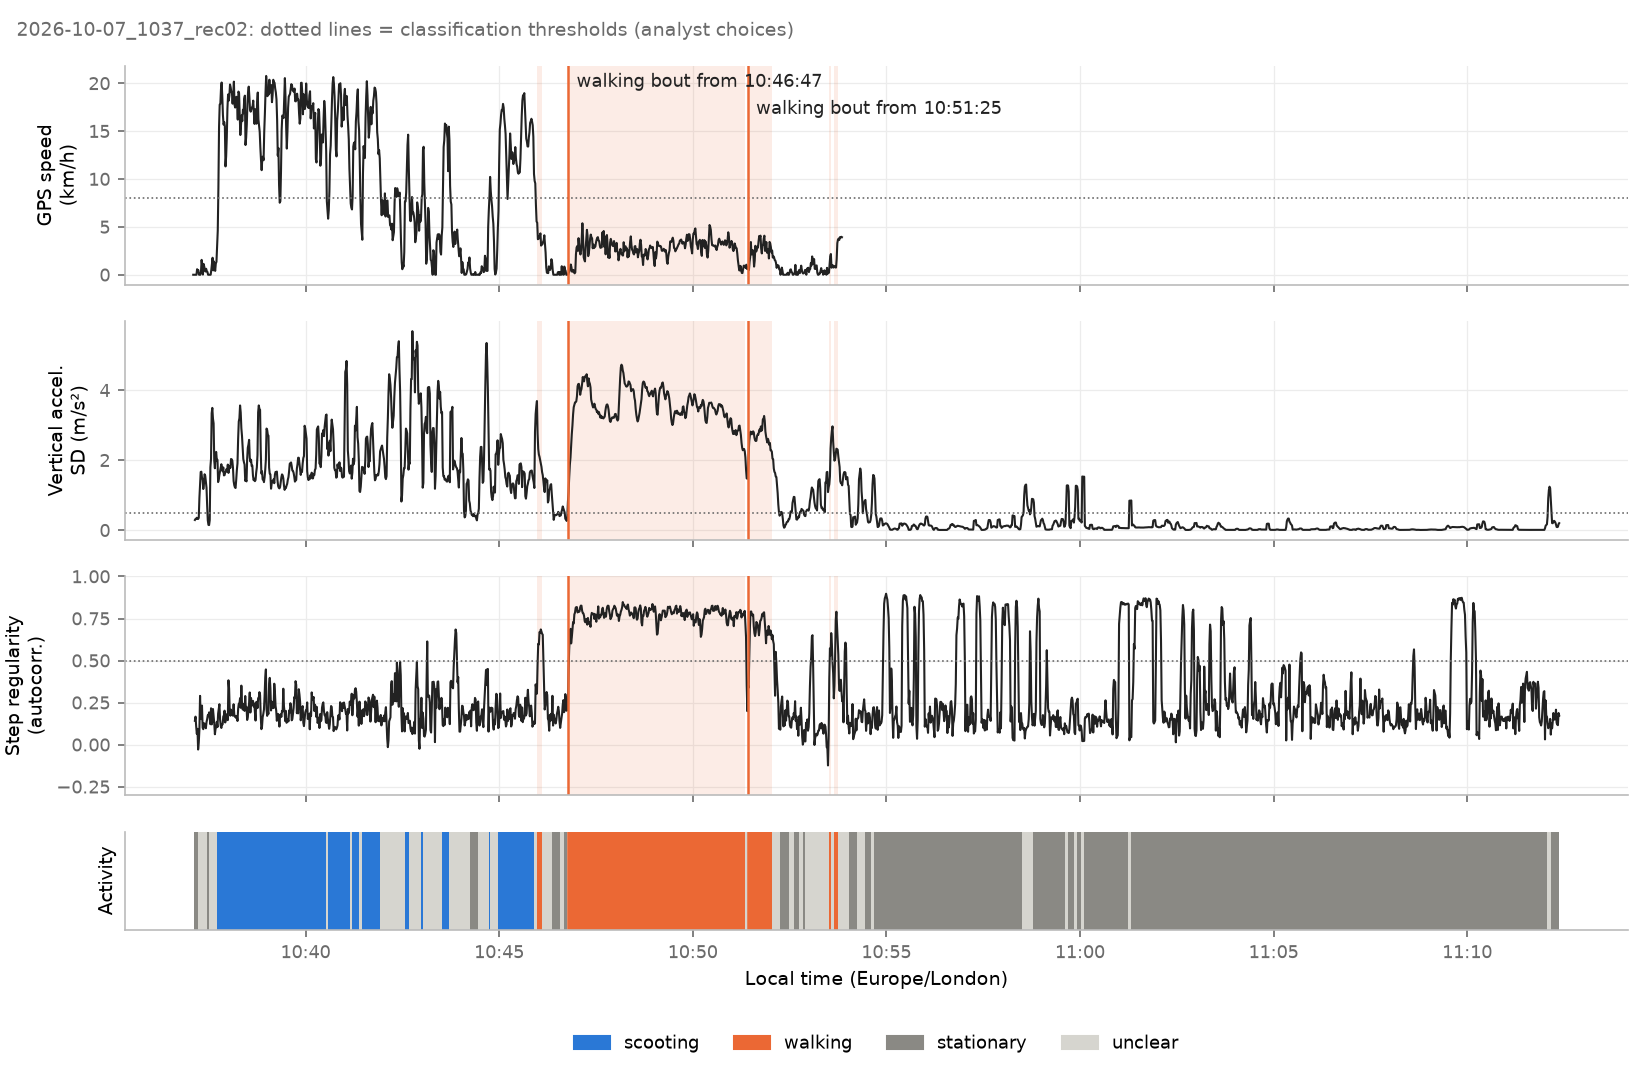
\includegraphics[width=\linewidth]{appendix/2026-10-07_1037_rec02_activity_timeline.png}
\caption{Ride 2: the ride, the walk from 10:46:47 and the phone at rest afterwards.
The repeated high step-regularity values after the walk come with almost no power in the
step band: a small periodic vibration, which the step-band rule correctly rejects.}\label{fig:B2}
\end{figure}

\begin{figure}[htbp]
\centering
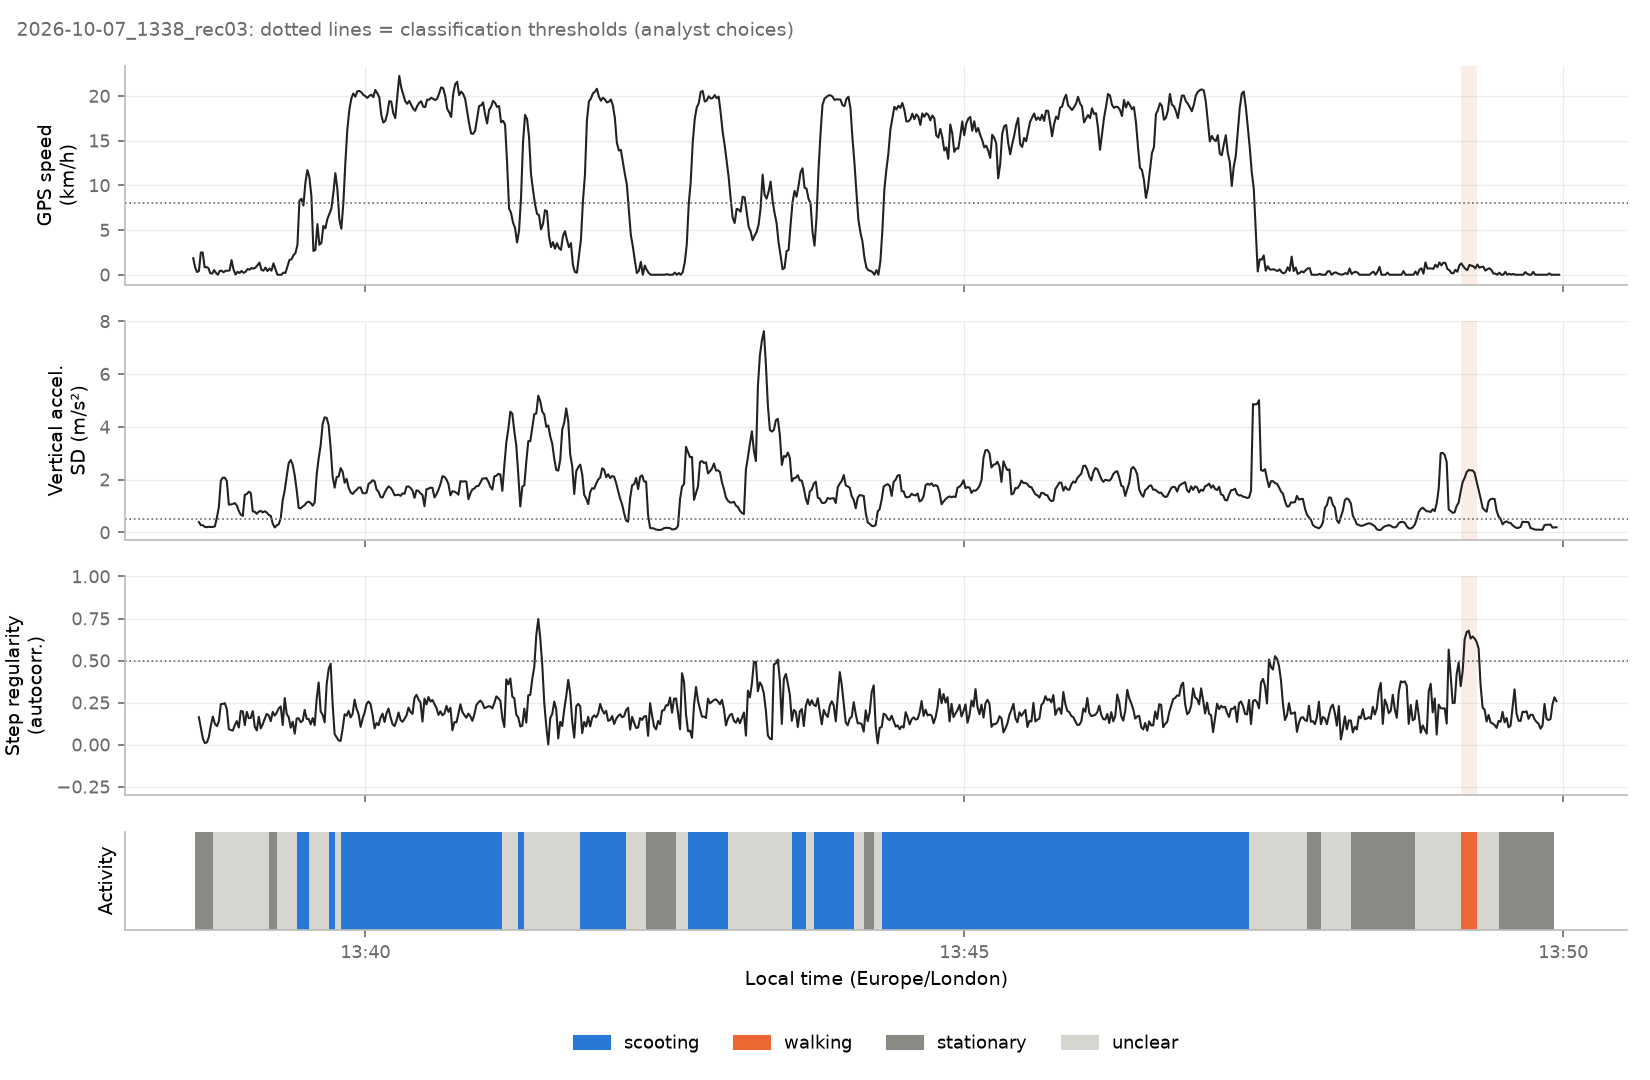
\includegraphics[width=\linewidth]{appendix/2026-10-07_1338_rec03_activity_timeline.png}
\caption{Ride 3.}\label{fig:B3}
\end{figure}


\section{Visual check of spots in street-level imagery}\label{visual-check-of-spots-in-street-level-imagery}

% SPOT_CHECK.md; outputs/combined/spot_links.csv

Table~\ref{tab:C1} lists the spots with links that open Google Street View at the spot,
facing the direction of travel and tilted 25° towards the road, a Google Maps pin, and
Mapillary imagery (the full list of all 33 spots, with the same links, is in the
supplementary file \texttt{spot\_links.csv}). The links use Google's documented Maps URLs,
which need no API key \autocite{googlemapsurls}; no imagery is downloaded, and no Street
View images are reproduced here, as Google does not permit their use in print. Open imagery was checked first:
Panoramax \autocite{panoramax} had no photos in the study area, and KartaView \autocite{kartaview} had
five photos near spot P1, from 2017 and 2021, too old to show the current surface.

Rules fixed before checking: record the imagery date shown in the viewer; record what is
visible within about 15 m of the spot (the phone's median GPS accuracy was 11--14 m) as
one or more of \emph{pothole}, \emph{crack or broken surface}, \emph{patched or repaired surface},
\emph{drain or manhole cover}, \emph{kerb or dropped kerb}, \emph{speed hump or raised table},
\emph{nothing visible}, \emph{no imagery}; do not change the categories once started. Imagery
dates differ from the ride dates, so a visible feature supports an impact but a clean
image does not rule a defect out.

\textbf{Results:} pending.

% Generated by scripts/paper_part_a.py (spot_table_tex) from outputs/combined/spot_links.csv;
% do not edit by hand. Styled after outputs/combined/spot_links.html.
\begin{landscape}
\footnotesize\arrayrulecolor{rulegray}
\setlength{\LTpre}{3pt}\setlength{\LTpost}{8pt}
\captionof{table}{Impact spots, most important first, as in the project's spot list. Links open Google Street View at the spot facing the direction of travel (tilted towards the road), a Google Maps pin, and Mapillary imagery. On paper, scan the QR code to open the same Street View, or enter the coordinates in any map. FixMyStreet: nearest road-surface report made in the 365 days before the ride (within 25 m, or the nearest). Spots P9, P16, P30, P31 lie in the hidden first or last 200 m of a route and are not listed, for privacy; they are included in all counts and in the tier totals.}\label{tab:C1}
\vspace{6pt}

\noindent{\normalsize\bfseries Tier 1: Hit on 2+ separate rides (10)}\par\nopagebreak
\begin{longtable}{@{}p{9mm} >{\raggedleft\arraybackslash}p{11mm} >{\raggedleft\arraybackslash}p{8mm} >{\raggedleft\arraybackslash}p{9mm} p{20mm} p{38mm} p{36mm} >{\raggedright\arraybackslash}p{31mm} >{\raggedright\arraybackslash}p{33mm} >{\centering\arraybackslash}p{14mm}@{}}
\toprule
Spot & Impacts & Rides & Max g & Road & Open & FixMyStreet (recent) & Location & Events (recording\#impact) & Scan \\
\midrule
\endfirsthead
\toprule
Spot & Impacts & Rides & Max g & Road & Open & FixMyStreet (recent) & Location & Events (recording\#impact) & Scan \\
\midrule
\endhead
\textbf{P1} & 6 & 3 & 2.24 & Marston Road & \href{https://www.google.com/maps/@?api=1\&map_action=pano\&viewpoint=51.754270,-1.235883\&heading=10\&pitch=-25\&fov=80}{Street View}\,\textperiodcentered\, \href{https://www.google.com/maps/search/?api=1\&query=51.754270,-1.235883}{Map}\,\textperiodcentered\, \href{https://www.mapillary.com/app/?lat=51.754270\&lng=-1.235883\&z=19}{Mapillary} & \textcolor{gray}{none $\leq$ 25 m (nearest \href{https://www.fixmystreet.com/report/9608286}{60 m})} & \textcolor{gray}{51.75427, −1.23588 \textperiodcentered{} \mbox{facing 10°}} & \textcolor{gray}{rec01\#31; rec02\#8; rec03\#17; rec03\#18; rec03\#19; rec03\#20} & \raisebox{-0.92\height}{\qrcode[height=13mm,level=L,nolink]{https://www.google.com/maps/@?api=1\&map_action=pano\&viewpoint=51.754270,-1.235883\&heading=10\&pitch=-25\&fov=80}} \\ \specialrule{0.2pt}{1pt}{1pt}
\textbf{P2} & 6 & 3 & 1.47 & Marston Road & \href{https://www.google.com/maps/@?api=1\&map_action=pano\&viewpoint=51.752684,-1.236654\&heading=27\&pitch=-25\&fov=80}{Street View}\,\textperiodcentered\, \href{https://www.google.com/maps/search/?api=1\&query=51.752684,-1.236654}{Map}\,\textperiodcentered\, \href{https://www.mapillary.com/app/?lat=51.752684\&lng=-1.236654\&z=19}{Mapillary} & \textcolor{gray}{none $\leq$ 25 m (nearest \href{https://www.fixmystreet.com/report/8694180}{44 m})} & \textcolor{gray}{51.75268, −1.23665 \textperiodcentered{} \mbox{facing 27°}} & \textcolor{gray}{rec01\#30; rec02\#9; rec02\#10; rec02\#11; rec02\#12; rec03\#16} & \raisebox{-0.92\height}{\qrcode[height=13mm,level=L,nolink]{https://www.google.com/maps/@?api=1\&map_action=pano\&viewpoint=51.752684,-1.236654\&heading=27\&pitch=-25\&fov=80}} \\ \specialrule{0.2pt}{1pt}{1pt}
\textbf{P3} & 19 & 2 & 2.25 & Other roads & \href{https://www.google.com/maps/@?api=1\&map_action=pano\&viewpoint=51.750235,-1.242534\&heading=261\&pitch=-25\&fov=80}{Street View}\,\textperiodcentered\, \href{https://www.google.com/maps/search/?api=1\&query=51.750235,-1.242534}{Map}\,\textperiodcentered\, \href{https://www.mapillary.com/app/?lat=51.750235\&lng=-1.242534\&z=19}{Mapillary} & report \href{https://www.fixmystreet.com/report/9029624}{5 m} (closed) & \textcolor{gray}{51.75024, −1.24253 \textperiodcentered{} \mbox{facing 261°}} & \textcolor{gray}{rec02\#25; rec02\#26; rec02\#27; rec02\#28; rec02\#29; rec02\#30; rec02\#31; rec02\#32; rec02\#33; rec02\#34; rec02\#35; rec02\#36; rec02\#37; rec02\#38; rec03\#1; rec03\#2; rec03\#3; rec03\#4; rec03\#5} & \raisebox{-0.92\height}{\qrcode[height=13mm,level=L,nolink]{https://www.google.com/maps/@?api=1\&map_action=pano\&viewpoint=51.750235,-1.242534\&heading=261\&pitch=-25\&fov=80}} \\ \specialrule{0.2pt}{1pt}{1pt}
\textbf{P4} & 10 & 2 & 6.28 & Other roads & \href{https://www.google.com/maps/@?api=1\&map_action=pano\&viewpoint=51.750849,-1.238775\&heading=218\&pitch=-25\&fov=80}{Street View}\,\textperiodcentered\, \href{https://www.google.com/maps/search/?api=1\&query=51.750849,-1.238775}{Map}\,\textperiodcentered\, \href{https://www.mapillary.com/app/?lat=51.750849\&lng=-1.238775\&z=19}{Mapillary} & report \href{https://www.fixmystreet.com/report/9436309}{8 m} (fixed) & \textcolor{gray}{51.75085, −1.23877 \textperiodcentered{} \mbox{facing 218°}} & \textcolor{gray}{rec02\#18; rec02\#19; rec02\#20; rec02\#21; rec02\#22; rec03\#9; rec03\#10; rec03\#11; rec03\#12; rec03\#13} & \raisebox{-0.92\height}{\qrcode[height=13mm,level=L,nolink]{https://www.google.com/maps/@?api=1\&map_action=pano\&viewpoint=51.750849,-1.238775\&heading=218\&pitch=-25\&fov=80}} \\ \specialrule{0.2pt}{1pt}{1pt}
\textbf{P5} & 9 & 2 & 1.79 & Marston Road & \href{https://www.google.com/maps/@?api=1\&map_action=pano\&viewpoint=51.756868,-1.235505\&heading=355\&pitch=-25\&fov=80}{Street View}\,\textperiodcentered\, \href{https://www.google.com/maps/search/?api=1\&query=51.756868,-1.235505}{Map}\,\textperiodcentered\, \href{https://www.mapillary.com/app/?lat=51.756868\&lng=-1.235505\&z=19}{Mapillary} & \textcolor{gray}{none $\leq$ 25 m (nearest \href{https://www.fixmystreet.com/report/9608286}{121 m})} & \textcolor{gray}{51.75687, −1.23551 \textperiodcentered{} \mbox{facing 355°}} & \textcolor{gray}{rec01\#33; rec01\#34; rec01\#35; rec01\#36; rec01\#37; rec02\#4; rec02\#5; rec02\#6; rec02\#7} & \raisebox{-0.92\height}{\qrcode[height=13mm,level=L,nolink]{https://www.google.com/maps/@?api=1\&map_action=pano\&viewpoint=51.756868,-1.235505\&heading=355\&pitch=-25\&fov=80}} \\ \specialrule{0.2pt}{1pt}{1pt}
\textbf{P6} & 4 & 2 & 1.85 & Other roads & \href{https://www.google.com/maps/@?api=1\&map_action=pano\&viewpoint=51.750594,-1.239934\&heading=249\&pitch=-25\&fov=80}{Street View}\,\textperiodcentered\, \href{https://www.google.com/maps/search/?api=1\&query=51.750594,-1.239934}{Map}\,\textperiodcentered\, \href{https://www.mapillary.com/app/?lat=51.750594\&lng=-1.239934\&z=19}{Mapillary} & report \href{https://www.fixmystreet.com/report/9850727}{8 m} (closed) & \textcolor{gray}{51.75059, −1.23993 \textperiodcentered{} \mbox{facing 249°}} & \textcolor{gray}{rec02\#23; rec02\#24; rec03\#7; rec03\#8} & \raisebox{-0.92\height}{\qrcode[height=13mm,level=L,nolink]{https://www.google.com/maps/@?api=1\&map_action=pano\&viewpoint=51.750594,-1.239934\&heading=249\&pitch=-25\&fov=80}} \\ \specialrule{0.2pt}{1pt}{1pt}
\textbf{P7} & 3 & 2 & 1.17 & Marston Road & \href{https://www.google.com/maps/@?api=1\&map_action=pano\&viewpoint=51.752081,-1.236996\&heading=180\&pitch=-25\&fov=80}{Street View}\,\textperiodcentered\, \href{https://www.google.com/maps/search/?api=1\&query=51.752081,-1.236996}{Map}\,\textperiodcentered\, \href{https://www.mapillary.com/app/?lat=51.752081\&lng=-1.236996\&z=19}{Mapillary} & report \href{https://www.fixmystreet.com/report/8512828}{8 m} (closed) & \textcolor{gray}{51.75208, −1.23700 \textperiodcentered{} \mbox{facing 180°}} & \textcolor{gray}{rec02\#13; rec02\#14; rec03\#15} & \raisebox{-0.92\height}{\qrcode[height=13mm,level=L,nolink]{https://www.google.com/maps/@?api=1\&map_action=pano\&viewpoint=51.752081,-1.236996\&heading=180\&pitch=-25\&fov=80}} \\ \specialrule{0.2pt}{1pt}{1pt}
\textbf{P8} & 2 & 2 & 2.80 & Other roads & \href{https://www.google.com/maps/@?api=1\&map_action=pano\&viewpoint=51.751550,-1.237717\&heading=52\&pitch=-25\&fov=80}{Street View}\,\textperiodcentered\, \href{https://www.google.com/maps/search/?api=1\&query=51.751550,-1.237717}{Map}\,\textperiodcentered\, \href{https://www.mapillary.com/app/?lat=51.751550\&lng=-1.237717\&z=19}{Mapillary} & \textcolor{gray}{none $\leq$ 25 m (nearest \href{https://www.fixmystreet.com/report/8336423}{38 m})} & \textcolor{gray}{51.75155, −1.23772 \textperiodcentered{} \mbox{facing 52°}} & \textcolor{gray}{rec01\#23; rec03\#14} & \raisebox{-0.92\height}{\qrcode[height=13mm,level=L,nolink]{https://www.google.com/maps/@?api=1\&map_action=pano\&viewpoint=51.751550,-1.237717\&heading=52\&pitch=-25\&fov=80}} \\ \specialrule{0.2pt}{1pt}{1pt}
\textbf{P10} & 2 & 2 & 1.34 & Marston Road & \href{https://www.google.com/maps/@?api=1\&map_action=pano\&viewpoint=51.757768,-1.235487\&heading=13\&pitch=-25\&fov=80}{Street View}\,\textperiodcentered\, \href{https://www.google.com/maps/search/?api=1\&query=51.757768,-1.235487}{Map}\,\textperiodcentered\, \href{https://www.mapillary.com/app/?lat=51.757768\&lng=-1.235487\&z=19}{Mapillary} & \textcolor{gray}{none $\leq$ 25 m (nearest \href{https://www.fixmystreet.com/report/8787376}{87 m})} & \textcolor{gray}{51.75777, −1.23549 \textperiodcentered{} \mbox{facing 13°}} & \textcolor{gray}{rec01\#38; rec03\#21} & \raisebox{-0.92\height}{\qrcode[height=13mm,level=L,nolink]{https://www.google.com/maps/@?api=1\&map_action=pano\&viewpoint=51.757768,-1.235487\&heading=13\&pitch=-25\&fov=80}} \\ \specialrule{0.2pt}{1pt}{1pt}
\end{longtable}

\needspace{9\baselineskip}
\noindent{\normalsize\bfseries Tier 2: 2+ impacts on one ride (10)}\par\nopagebreak
\begin{longtable}{@{}p{9mm} >{\raggedleft\arraybackslash}p{11mm} >{\raggedleft\arraybackslash}p{8mm} >{\raggedleft\arraybackslash}p{9mm} p{20mm} p{38mm} p{36mm} >{\raggedright\arraybackslash}p{31mm} >{\raggedright\arraybackslash}p{33mm} >{\centering\arraybackslash}p{14mm}@{}}
\toprule
Spot & Impacts & Rides & Max g & Road & Open & FixMyStreet (recent) & Location & Events (recording\#impact) & Scan \\
\midrule
\endfirsthead
\toprule
Spot & Impacts & Rides & Max g & Road & Open & FixMyStreet (recent) & Location & Events (recording\#impact) & Scan \\
\midrule
\endhead
\textbf{P11} & 3 & 1 & 2.87 & Morrell Avenue & \href{https://www.google.com/maps/@?api=1\&map_action=pano\&viewpoint=51.751237,-1.237962\&heading=224\&pitch=-25\&fov=80}{Street View}\,\textperiodcentered\, \href{https://www.google.com/maps/search/?api=1\&query=51.751237,-1.237962}{Map}\,\textperiodcentered\, \href{https://www.mapillary.com/app/?lat=51.751237\&lng=-1.237962\&z=19}{Mapillary} & report \href{https://www.fixmystreet.com/report/9495439}{12 m} (closed) & \textcolor{gray}{51.75124, −1.23796 \textperiodcentered{} \mbox{facing 224°}} & \textcolor{gray}{rec02\#15; rec02\#16; rec02\#17} & \raisebox{-0.92\height}{\qrcode[height=13mm,level=L,nolink]{https://www.google.com/maps/@?api=1\&map_action=pano\&viewpoint=51.751237,-1.237962\&heading=224\&pitch=-25\&fov=80}} \\ \specialrule{0.2pt}{1pt}{1pt}
\textbf{P12} & 3 & 1 & 2.68 & Other roads & \href{https://www.google.com/maps/@?api=1\&map_action=pano\&viewpoint=51.752220,-1.237662\&heading=286\&pitch=-25\&fov=80}{Street View}\,\textperiodcentered\, \href{https://www.google.com/maps/search/?api=1\&query=51.752220,-1.237662}{Map}\,\textperiodcentered\, \href{https://www.mapillary.com/app/?lat=51.752220\&lng=-1.237662\&z=19}{Mapillary} & report \href{https://www.fixmystreet.com/report/8666347}{6 m} (fixed) & \textcolor{gray}{51.75222, −1.23766 \textperiodcentered{} \mbox{facing 286°}} & \textcolor{gray}{rec01\#24; rec01\#28; rec01\#29} & \raisebox{-0.92\height}{\qrcode[height=13mm,level=L,nolink]{https://www.google.com/maps/@?api=1\&map_action=pano\&viewpoint=51.752220,-1.237662\&heading=286\&pitch=-25\&fov=80}} \\ \specialrule{0.2pt}{1pt}{1pt}
\textbf{P13} & 3 & 1 & 1.48 & Morrell Avenue & \href{https://www.google.com/maps/@?api=1\&map_action=pano\&viewpoint=51.749809,-1.230171\&heading=267\&pitch=-25\&fov=80}{Street View}\,\textperiodcentered\, \href{https://www.google.com/maps/search/?api=1\&query=51.749809,-1.230171}{Map}\,\textperiodcentered\, \href{https://www.mapillary.com/app/?lat=51.749809\&lng=-1.230171\&z=19}{Mapillary} & \textcolor{gray}{none $\leq$ 25 m (nearest \href{https://www.fixmystreet.com/report/9012527}{113 m})} & \textcolor{gray}{51.74981, −1.23017 \textperiodcentered{} \mbox{facing 267°}} & \textcolor{gray}{rec01\#13; rec01\#14; rec01\#15} & \raisebox{-0.92\height}{\qrcode[height=13mm,level=L,nolink]{https://www.google.com/maps/@?api=1\&map_action=pano\&viewpoint=51.749809,-1.230171\&heading=267\&pitch=-25\&fov=80}} \\ \specialrule{0.2pt}{1pt}{1pt}
\textbf{P14} & 3 & 1 & 1.17 & Other roads & \href{https://www.google.com/maps/@?api=1\&map_action=pano\&viewpoint=51.751621,-1.222891\&heading=226\&pitch=-25\&fov=80}{Street View}\,\textperiodcentered\, \href{https://www.google.com/maps/search/?api=1\&query=51.751621,-1.222891}{Map}\,\textperiodcentered\, \href{https://www.mapillary.com/app/?lat=51.751621\&lng=-1.222891\&z=19}{Mapillary} & \textcolor{gray}{none $\leq$ 25 m (nearest \href{https://www.fixmystreet.com/report/8744515}{118 m})} & \textcolor{gray}{51.75162, −1.22289 \textperiodcentered{} \mbox{facing 226°}} & \textcolor{gray}{rec01\#6; rec01\#7; rec01\#8} & \raisebox{-0.92\height}{\qrcode[height=13mm,level=L,nolink]{https://www.google.com/maps/@?api=1\&map_action=pano\&viewpoint=51.751621,-1.222891\&heading=226\&pitch=-25\&fov=80}} \\ \specialrule{0.2pt}{1pt}{1pt}
\textbf{P15} & 2 & 1 & 1.37 & Other roads & \href{https://www.google.com/maps/@?api=1\&map_action=pano\&viewpoint=51.752562,-1.238892\&heading=293\&pitch=-25\&fov=80}{Street View}\,\textperiodcentered\, \href{https://www.google.com/maps/search/?api=1\&query=51.752562,-1.238892}{Map}\,\textperiodcentered\, \href{https://www.mapillary.com/app/?lat=51.752562\&lng=-1.238892\&z=19}{Mapillary} & \textcolor{gray}{none $\leq$ 25 m (nearest \href{https://www.fixmystreet.com/report/8666347}{73 m})} & \textcolor{gray}{51.75256, −1.23889 \textperiodcentered{} \mbox{facing 293°}} & \textcolor{gray}{rec01\#25; rec01\#26} & \raisebox{-0.92\height}{\qrcode[height=13mm,level=L,nolink]{https://www.google.com/maps/@?api=1\&map_action=pano\&viewpoint=51.752562,-1.238892\&heading=293\&pitch=-25\&fov=80}} \\ \specialrule{0.2pt}{1pt}{1pt}
\textbf{P17} & 2 & 1 & 1.31 & Morrell Avenue & \href{https://www.google.com/maps/@?api=1\&map_action=pano\&viewpoint=51.749740,-1.231359\&heading=265\&pitch=-25\&fov=80}{Street View}\,\textperiodcentered\, \href{https://www.google.com/maps/search/?api=1\&query=51.749740,-1.231359}{Map}\,\textperiodcentered\, \href{https://www.mapillary.com/app/?lat=51.749740\&lng=-1.231359\&z=19}{Mapillary} & \textcolor{gray}{none $\leq$ 25 m (nearest \href{https://www.fixmystreet.com/report/9012527}{178 m})} & \textcolor{gray}{51.74974, −1.23136 \textperiodcentered{} \mbox{facing 265°}} & \textcolor{gray}{rec01\#16; rec01\#17} & \raisebox{-0.92\height}{\qrcode[height=13mm,level=L,nolink]{https://www.google.com/maps/@?api=1\&map_action=pano\&viewpoint=51.749740,-1.231359\&heading=265\&pitch=-25\&fov=80}} \\ \specialrule{0.2pt}{1pt}{1pt}
\textbf{P18} & 2 & 1 & 1.24 & Other roads & \href{https://www.google.com/maps/@?api=1\&map_action=pano\&viewpoint=51.751195,-1.223560\&heading=224\&pitch=-25\&fov=80}{Street View}\,\textperiodcentered\, \href{https://www.google.com/maps/search/?api=1\&query=51.751195,-1.223560}{Map}\,\textperiodcentered\, \href{https://www.mapillary.com/app/?lat=51.751195\&lng=-1.223560\&z=19}{Mapillary} & \textcolor{gray}{none $\leq$ 25 m (nearest \href{https://www.fixmystreet.com/report/9236232}{115 m})} & \textcolor{gray}{51.75120, −1.22356 \textperiodcentered{} \mbox{facing 224°}} & \textcolor{gray}{rec01\#9; rec01\#10} & \raisebox{-0.92\height}{\qrcode[height=13mm,level=L,nolink]{https://www.google.com/maps/@?api=1\&map_action=pano\&viewpoint=51.751195,-1.223560\&heading=224\&pitch=-25\&fov=80}} \\ \specialrule{0.2pt}{1pt}{1pt}
\textbf{P19} & 2 & 1 & 1.18 & Morrell Avenue & \href{https://www.google.com/maps/@?api=1\&map_action=pano\&viewpoint=51.749830,-1.233869\&heading=285\&pitch=-25\&fov=80}{Street View}\,\textperiodcentered\, \href{https://www.google.com/maps/search/?api=1\&query=51.749830,-1.233869}{Map}\,\textperiodcentered\, \href{https://www.mapillary.com/app/?lat=51.749830\&lng=-1.233869\&z=19}{Mapillary} & \textcolor{gray}{none $\leq$ 25 m (nearest \href{https://www.fixmystreet.com/report/9415948}{75 m})} & \textcolor{gray}{51.74983, −1.23387 \textperiodcentered{} \mbox{facing 285°}} & \textcolor{gray}{rec01\#18; rec01\#19} & \raisebox{-0.92\height}{\qrcode[height=13mm,level=L,nolink]{https://www.google.com/maps/@?api=1\&map_action=pano\&viewpoint=51.749830,-1.233869\&heading=285\&pitch=-25\&fov=80}} \\ \specialrule{0.2pt}{1pt}{1pt}
\textbf{P20} & 2 & 1 & 1.13 & Old Road & \href{https://www.google.com/maps/@?api=1\&map_action=pano\&viewpoint=51.753330,-1.218484\&heading=248\&pitch=-25\&fov=80}{Street View}\,\textperiodcentered\, \href{https://www.google.com/maps/search/?api=1\&query=51.753330,-1.218484}{Map}\,\textperiodcentered\, \href{https://www.mapillary.com/app/?lat=51.753330\&lng=-1.218484\&z=19}{Mapillary} & \textcolor{gray}{none $\leq$ 25 m (nearest \href{https://www.fixmystreet.com/report/8852037}{58 m})} & \textcolor{gray}{51.75333, −1.21848 \textperiodcentered{} \mbox{facing 248°}} & \textcolor{gray}{rec01\#3; rec01\#4} & \raisebox{-0.92\height}{\qrcode[height=13mm,level=L,nolink]{https://www.google.com/maps/@?api=1\&map_action=pano\&viewpoint=51.753330,-1.218484\&heading=248\&pitch=-25\&fov=80}} \\ \specialrule{0.2pt}{1pt}{1pt}
\end{longtable}

\needspace{9\baselineskip}
\noindent{\normalsize\bfseries Tier 3: Single impact (13)}\par\nopagebreak
\begin{longtable}{@{}p{9mm} >{\raggedleft\arraybackslash}p{11mm} >{\raggedleft\arraybackslash}p{8mm} >{\raggedleft\arraybackslash}p{9mm} p{20mm} p{38mm} p{36mm} >{\raggedright\arraybackslash}p{31mm} >{\raggedright\arraybackslash}p{33mm} >{\centering\arraybackslash}p{14mm}@{}}
\toprule
Spot & Impacts & Rides & Max g & Road & Open & FixMyStreet (recent) & Location & Events (recording\#impact) & Scan \\
\midrule
\endfirsthead
\toprule
Spot & Impacts & Rides & Max g & Road & Open & FixMyStreet (recent) & Location & Events (recording\#impact) & Scan \\
\midrule
\endhead
\textbf{P21} & 1 & 1 & 2.64 & Other roads & \href{https://www.google.com/maps/@?api=1\&map_action=pano\&viewpoint=51.749873,-1.244328\&heading=219\&pitch=-25\&fov=80}{Street View}\,\textperiodcentered\, \href{https://www.google.com/maps/search/?api=1\&query=51.749873,-1.244328}{Map}\,\textperiodcentered\, \href{https://www.mapillary.com/app/?lat=51.749873\&lng=-1.244328\&z=19}{Mapillary} & report \href{https://www.fixmystreet.com/report/8891248}{23 m} (fixed) & \textcolor{gray}{51.74987, −1.24433 \textperiodcentered{} \mbox{facing 219°}} & \textcolor{gray}{rec02\#39} & \raisebox{-0.92\height}{\qrcode[height=13mm,level=L,nolink]{https://www.google.com/maps/@?api=1\&map_action=pano\&viewpoint=51.749873,-1.244328\&heading=219\&pitch=-25\&fov=80}} \\ \specialrule{0.2pt}{1pt}{1pt}
\textbf{P22} & 1 & 1 & 1.73 & Other roads & \href{https://www.google.com/maps/@?api=1\&map_action=pano\&viewpoint=51.752107,-1.222087\&heading=225\&pitch=-25\&fov=80}{Street View}\,\textperiodcentered\, \href{https://www.google.com/maps/search/?api=1\&query=51.752107,-1.222087}{Map}\,\textperiodcentered\, \href{https://www.mapillary.com/app/?lat=51.752107\&lng=-1.222087\&z=19}{Mapillary} & \textcolor{gray}{none $\leq$ 25 m (nearest \href{https://www.fixmystreet.com/report/8744515}{52 m})} & \textcolor{gray}{51.75211, −1.22209 \textperiodcentered{} \mbox{facing 225°}} & \textcolor{gray}{rec01\#5} & \raisebox{-0.92\height}{\qrcode[height=13mm,level=L,nolink]{https://www.google.com/maps/@?api=1\&map_action=pano\&viewpoint=51.752107,-1.222087\&heading=225\&pitch=-25\&fov=80}} \\ \specialrule{0.2pt}{1pt}{1pt}
\textbf{P23} & 1 & 1 & 1.39 & Marston Road & \href{https://www.google.com/maps/@?api=1\&map_action=pano\&viewpoint=51.755210,-1.235670\&heading=8\&pitch=-25\&fov=80}{Street View}\,\textperiodcentered\, \href{https://www.google.com/maps/search/?api=1\&query=51.755210,-1.235670}{Map}\,\textperiodcentered\, \href{https://www.mapillary.com/app/?lat=51.755210\&lng=-1.235670\&z=19}{Mapillary} & report \href{https://www.fixmystreet.com/report/9608286}{5 m} (closed) & \textcolor{gray}{51.75521, −1.23567 \textperiodcentered{} \mbox{facing 8°}} & \textcolor{gray}{rec01\#32} & \raisebox{-0.92\height}{\qrcode[height=13mm,level=L,nolink]{https://www.google.com/maps/@?api=1\&map_action=pano\&viewpoint=51.755210,-1.235670\&heading=8\&pitch=-25\&fov=80}} \\ \specialrule{0.2pt}{1pt}{1pt}
\textbf{P24} & 1 & 1 & 1.23 & Morrell Avenue & \href{https://www.google.com/maps/@?api=1\&map_action=pano\&viewpoint=51.750129,-1.235206\&heading=308\&pitch=-25\&fov=80}{Street View}\,\textperiodcentered\, \href{https://www.google.com/maps/search/?api=1\&query=51.750129,-1.235206}{Map}\,\textperiodcentered\, \href{https://www.mapillary.com/app/?lat=51.750129\&lng=-1.235206\&z=19}{Mapillary} & \textcolor{gray}{none $\leq$ 25 m (nearest \href{https://www.fixmystreet.com/report/9415948}{73 m})} & \textcolor{gray}{51.75013, −1.23521 \textperiodcentered{} \mbox{facing 308°}} & \textcolor{gray}{rec01\#20} & \raisebox{-0.92\height}{\qrcode[height=13mm,level=L,nolink]{https://www.google.com/maps/@?api=1\&map_action=pano\&viewpoint=51.750129,-1.235206\&heading=308\&pitch=-25\&fov=80}} \\ \specialrule{0.2pt}{1pt}{1pt}
\textbf{P25} & 1 & 1 & 1.19 & Morrell Avenue & \href{https://www.google.com/maps/@?api=1\&map_action=pano\&viewpoint=51.750147,-1.226823\&heading=251\&pitch=-25\&fov=80}{Street View}\,\textperiodcentered\, \href{https://www.google.com/maps/search/?api=1\&query=51.750147,-1.226823}{Map}\,\textperiodcentered\, \href{https://www.mapillary.com/app/?lat=51.750147\&lng=-1.226823\&z=19}{Mapillary} & \textcolor{gray}{none $\leq$ 25 m (nearest \href{https://www.fixmystreet.com/report/8659259}{115 m})} & \textcolor{gray}{51.75015, −1.22682 \textperiodcentered{} \mbox{facing 251°}} & \textcolor{gray}{rec01\#11} & \raisebox{-0.92\height}{\qrcode[height=13mm,level=L,nolink]{https://www.google.com/maps/@?api=1\&map_action=pano\&viewpoint=51.750147,-1.226823\&heading=251\&pitch=-25\&fov=80}} \\ \specialrule{0.2pt}{1pt}{1pt}
\textbf{P26} & 1 & 1 & 1.17 & Other roads & \href{https://www.google.com/maps/@?api=1\&map_action=pano\&viewpoint=51.752416,-1.238294\&heading=111\&pitch=-25\&fov=80}{Street View}\,\textperiodcentered\, \href{https://www.google.com/maps/search/?api=1\&query=51.752416,-1.238294}{Map}\,\textperiodcentered\, \href{https://www.mapillary.com/app/?lat=51.752416\&lng=-1.238294\&z=19}{Mapillary} & \textcolor{gray}{none $\leq$ 25 m (nearest \href{https://www.fixmystreet.com/report/8666347}{31 m})} & \textcolor{gray}{51.75242, −1.23829 \textperiodcentered{} \mbox{facing 111°}} & \textcolor{gray}{rec01\#27} & \raisebox{-0.92\height}{\qrcode[height=13mm,level=L,nolink]{https://www.google.com/maps/@?api=1\&map_action=pano\&viewpoint=51.752416,-1.238294\&heading=111\&pitch=-25\&fov=80}} \\ \specialrule{0.2pt}{1pt}{1pt}
\textbf{P27} & 1 & 1 & 1.15 & Marston Road & \href{https://www.google.com/maps/@?api=1\&map_action=pano\&viewpoint=51.758061,-1.235642\&heading=176\&pitch=-25\&fov=80}{Street View}\,\textperiodcentered\, \href{https://www.google.com/maps/search/?api=1\&query=51.758061,-1.235642}{Map}\,\textperiodcentered\, \href{https://www.mapillary.com/app/?lat=51.758061\&lng=-1.235642\&z=19}{Mapillary} & \textcolor{gray}{none $\leq$ 25 m (nearest \href{https://www.fixmystreet.com/report/9020598}{249 m})} & \textcolor{gray}{51.75806, −1.23564 \textperiodcentered{} \mbox{facing 176°}} & \textcolor{gray}{rec02\#3} & \raisebox{-0.92\height}{\qrcode[height=13mm,level=L,nolink]{https://www.google.com/maps/@?api=1\&map_action=pano\&viewpoint=51.758061,-1.235642\&heading=176\&pitch=-25\&fov=80}} \\ \specialrule{0.2pt}{1pt}{1pt}
\textbf{P28} & 1 & 1 & 1.13 & Morrell Avenue & \href{https://www.google.com/maps/@?api=1\&map_action=pano\&viewpoint=51.750307,-1.235572\&heading=304\&pitch=-25\&fov=80}{Street View}\,\textperiodcentered\, \href{https://www.google.com/maps/search/?api=1\&query=51.750307,-1.235572}{Map}\,\textperiodcentered\, \href{https://www.mapillary.com/app/?lat=51.750307\&lng=-1.235572\&z=19}{Mapillary} & \textcolor{gray}{none $\leq$ 25 m (nearest \href{https://www.fixmystreet.com/report/8668106}{68 m})} & \textcolor{gray}{51.75031, −1.23557 \textperiodcentered{} \mbox{facing 304°}} & \textcolor{gray}{rec01\#21} & \raisebox{-0.92\height}{\qrcode[height=13mm,level=L,nolink]{https://www.google.com/maps/@?api=1\&map_action=pano\&viewpoint=51.750307,-1.235572\&heading=304\&pitch=-25\&fov=80}} \\ \specialrule{0.2pt}{1pt}{1pt}
\textbf{P29} & 1 & 1 & 1.12 & Morrell Avenue & \href{https://www.google.com/maps/@?api=1\&map_action=pano\&viewpoint=51.750943,-1.236971\&heading=297\&pitch=-25\&fov=80}{Street View}\,\textperiodcentered\, \href{https://www.google.com/maps/search/?api=1\&query=51.750943,-1.236971}{Map}\,\textperiodcentered\, \href{https://www.mapillary.com/app/?lat=51.750943\&lng=-1.236971\&z=19}{Mapillary} & \textcolor{gray}{none $\leq$ 25 m (nearest \href{https://www.fixmystreet.com/report/9052222}{65 m})} & \textcolor{gray}{51.75094, −1.23697 \textperiodcentered{} \mbox{facing 297°}} & \textcolor{gray}{rec01\#22} & \raisebox{-0.92\height}{\qrcode[height=13mm,level=L,nolink]{https://www.google.com/maps/@?api=1\&map_action=pano\&viewpoint=51.750943,-1.236971\&heading=297\&pitch=-25\&fov=80}} \\ \specialrule{0.2pt}{1pt}{1pt}
\textbf{P32} & 1 & 1 & 1.05 & Other roads & \href{https://www.google.com/maps/@?api=1\&map_action=pano\&viewpoint=51.750375,-1.241276\&heading=80\&pitch=-25\&fov=80}{Street View}\,\textperiodcentered\, \href{https://www.google.com/maps/search/?api=1\&query=51.750375,-1.241276}{Map}\,\textperiodcentered\, \href{https://www.mapillary.com/app/?lat=51.750375\&lng=-1.241276\&z=19}{Mapillary} & \textcolor{gray}{none $\leq$ 25 m (nearest \href{https://www.fixmystreet.com/report/10069088}{68 m})} & \textcolor{gray}{51.75037, −1.24128 \textperiodcentered{} \mbox{facing 80°}} & \textcolor{gray}{rec03\#6} & \raisebox{-0.92\height}{\qrcode[height=13mm,level=L,nolink]{https://www.google.com/maps/@?api=1\&map_action=pano\&viewpoint=51.750375,-1.241276\&heading=80\&pitch=-25\&fov=80}} \\ \specialrule{0.2pt}{1pt}{1pt}
\textbf{P33} & 1 & 1 & 1.04 & Morrell Avenue & \href{https://www.google.com/maps/@?api=1\&map_action=pano\&viewpoint=51.750045,-1.227441\&heading=260\&pitch=-25\&fov=80}{Street View}\,\textperiodcentered\, \href{https://www.google.com/maps/search/?api=1\&query=51.750045,-1.227441}{Map}\,\textperiodcentered\, \href{https://www.mapillary.com/app/?lat=51.750045\&lng=-1.227441\&z=19}{Mapillary} & \textcolor{gray}{none $\leq$ 25 m (nearest \href{https://www.fixmystreet.com/report/9012527}{131 m})} & \textcolor{gray}{51.75005, −1.22744 \textperiodcentered{} \mbox{facing 260°}} & \textcolor{gray}{rec01\#12} & \raisebox{-0.92\height}{\qrcode[height=13mm,level=L,nolink]{https://www.google.com/maps/@?api=1\&map_action=pano\&viewpoint=51.750045,-1.227441\&heading=260\&pitch=-25\&fov=80}} \\ \specialrule{0.2pt}{1pt}{1pt}
\end{longtable}

\arrayrulecolor{black}
\end{landscape}


% TODO: summarise outputs/combined/spot_links.csv by tier once checked
